\documentclass[a4paper,10pt]{article}
\usepackage[utf8]{inputenc}

\usepackage{graphicx}
\usepackage{float}
%opening
\title{Preliminary data analytics on genomic breaks}
\author{Dario Garcia-Gasulla, in collaboration with David Torrents,\\ Luisa Delgado, Juan Blanco Heredia, Armand Viltalta and \\Ferran Par\'{e}s. }

\begin{document}

\maketitle


\section*{Data overview}

Data is obtained from 556 patients, with the corresponding breaks. Patients have been found to have chromoplexy. All patients are considered as independent instances, and all breaks as independent variables. Each break has a source or target, which simply identifies an arbitrary order of break. There are 5 types of breaks as provided by the .vcf.tsv files: h2hINV, DEL, t2tINV, DUP, TRA.


\section*{Chromosome break distribution}

\subsection*{Distribution of breaks}

First we plot the number of breaks per chromosome, regardless of type.

\begin{figure}[H]
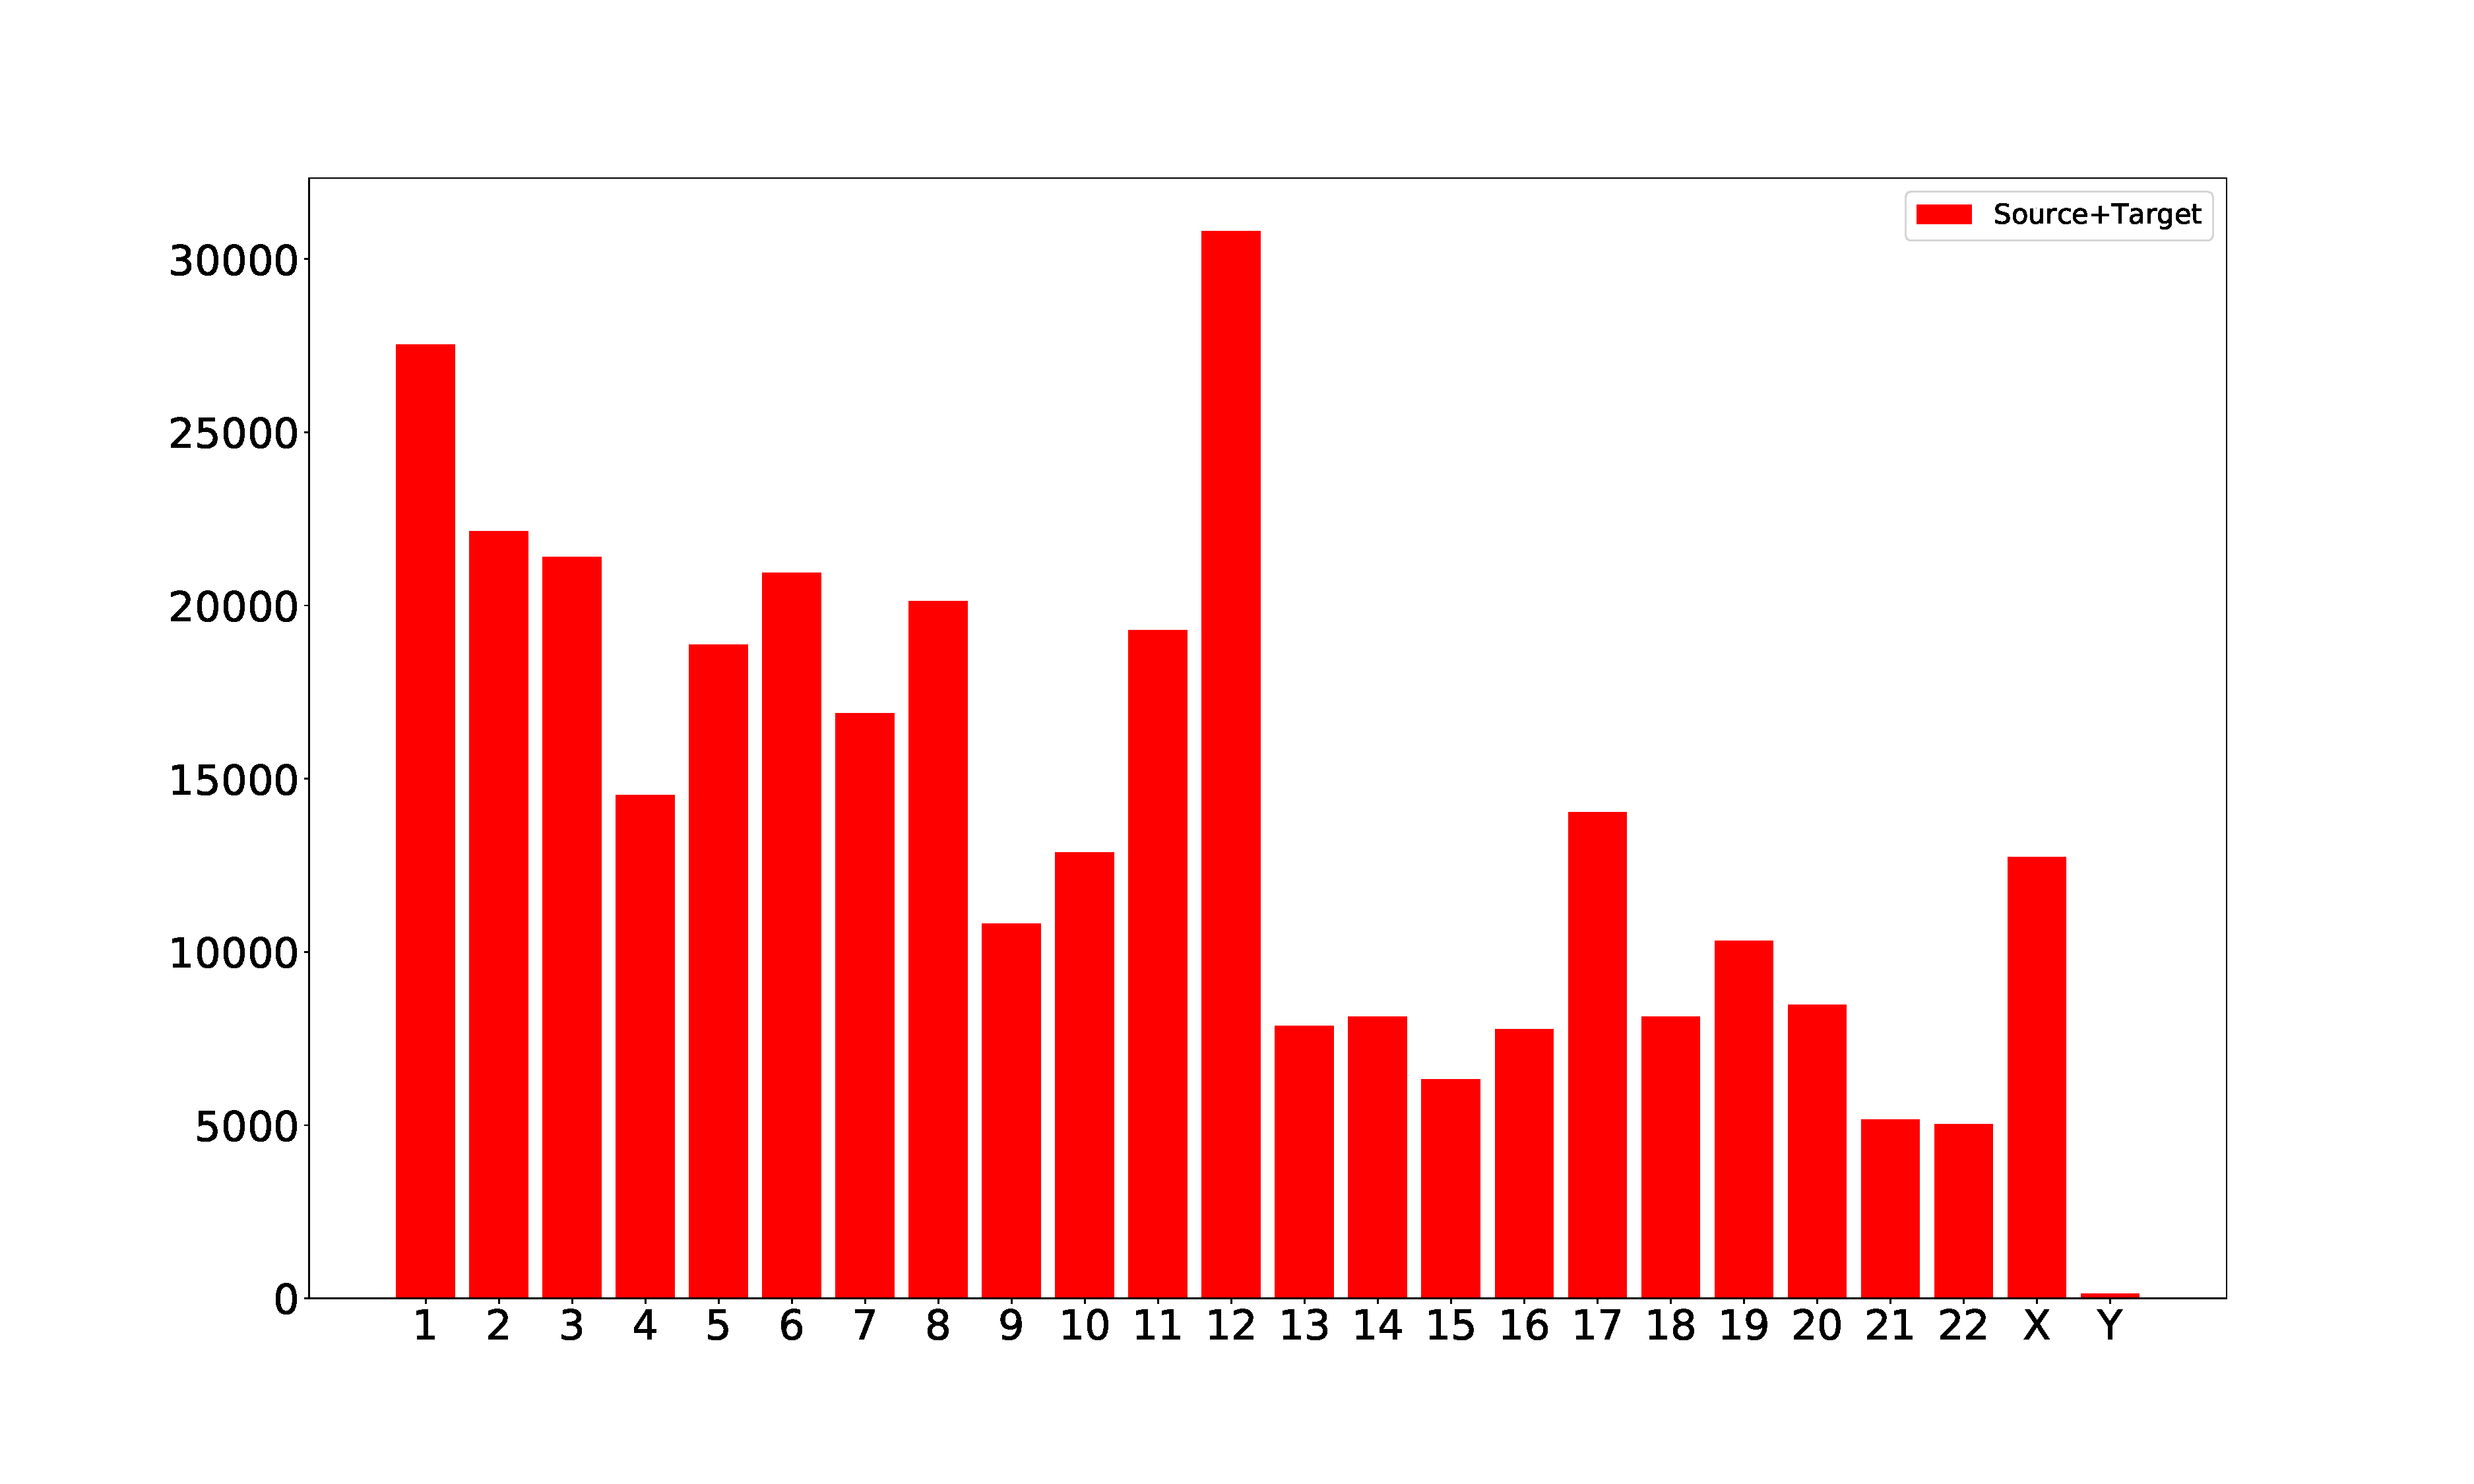
\includegraphics[scale=0.2]{figures/All_Break_distribution_unnormalized.pdf}
\caption{Distribution of breaks per chromosome. All brake types are aggregated. Values not normalized}
\end{figure}

We normalize by chromosome length, using the following lengths (from https://en.wikipedia.org/wiki/Human\_genome):
\begin{itemize}
\item chromosome\_size['1'] =  248956422.0
\item chromosome\_size['2'] =  242193529.0
\item chromosome\_size['3'] =  198295559.0
\item chromosome\_size['4'] =  190214555.0
\item chromosome\_size['5'] =  181538259.0
\item chromosome\_size['6'] =  170805979.0
\item chromosome\_size['7'] =  159345973.0
\item chromosome\_size['8'] =  145138636.0
\item chromosome\_size['9'] =  138394717.0
\item chromosome\_size['10'] = 133797422.0
\item chromosome\_size['11'] = 135086622.0
\item chromosome\_size['12'] = 133275309.0
\item chromosome\_size['13'] = 114364328.0
\item chromosome\_size['14'] = 107043718.0
\item chromosome\_size['15'] = 101991189.0
\item chromosome\_size['16'] = 90338345.0
\item chromosome\_size['17'] = 83257441.0
\item chromosome\_size['18'] = 80373285.0
\item chromosome\_size['19'] = 58617616.0
\item chromosome\_size['20'] = 64444167.0
\item chromosome\_size['21'] = 46709983.0
\item chromosome\_size['22'] = 50818468.0
\item chromosome\_size['X'] =  156040895.0
\item chromosome\_size['Y'] =  57227415.0
\end{itemize}

\begin{figure}[H]
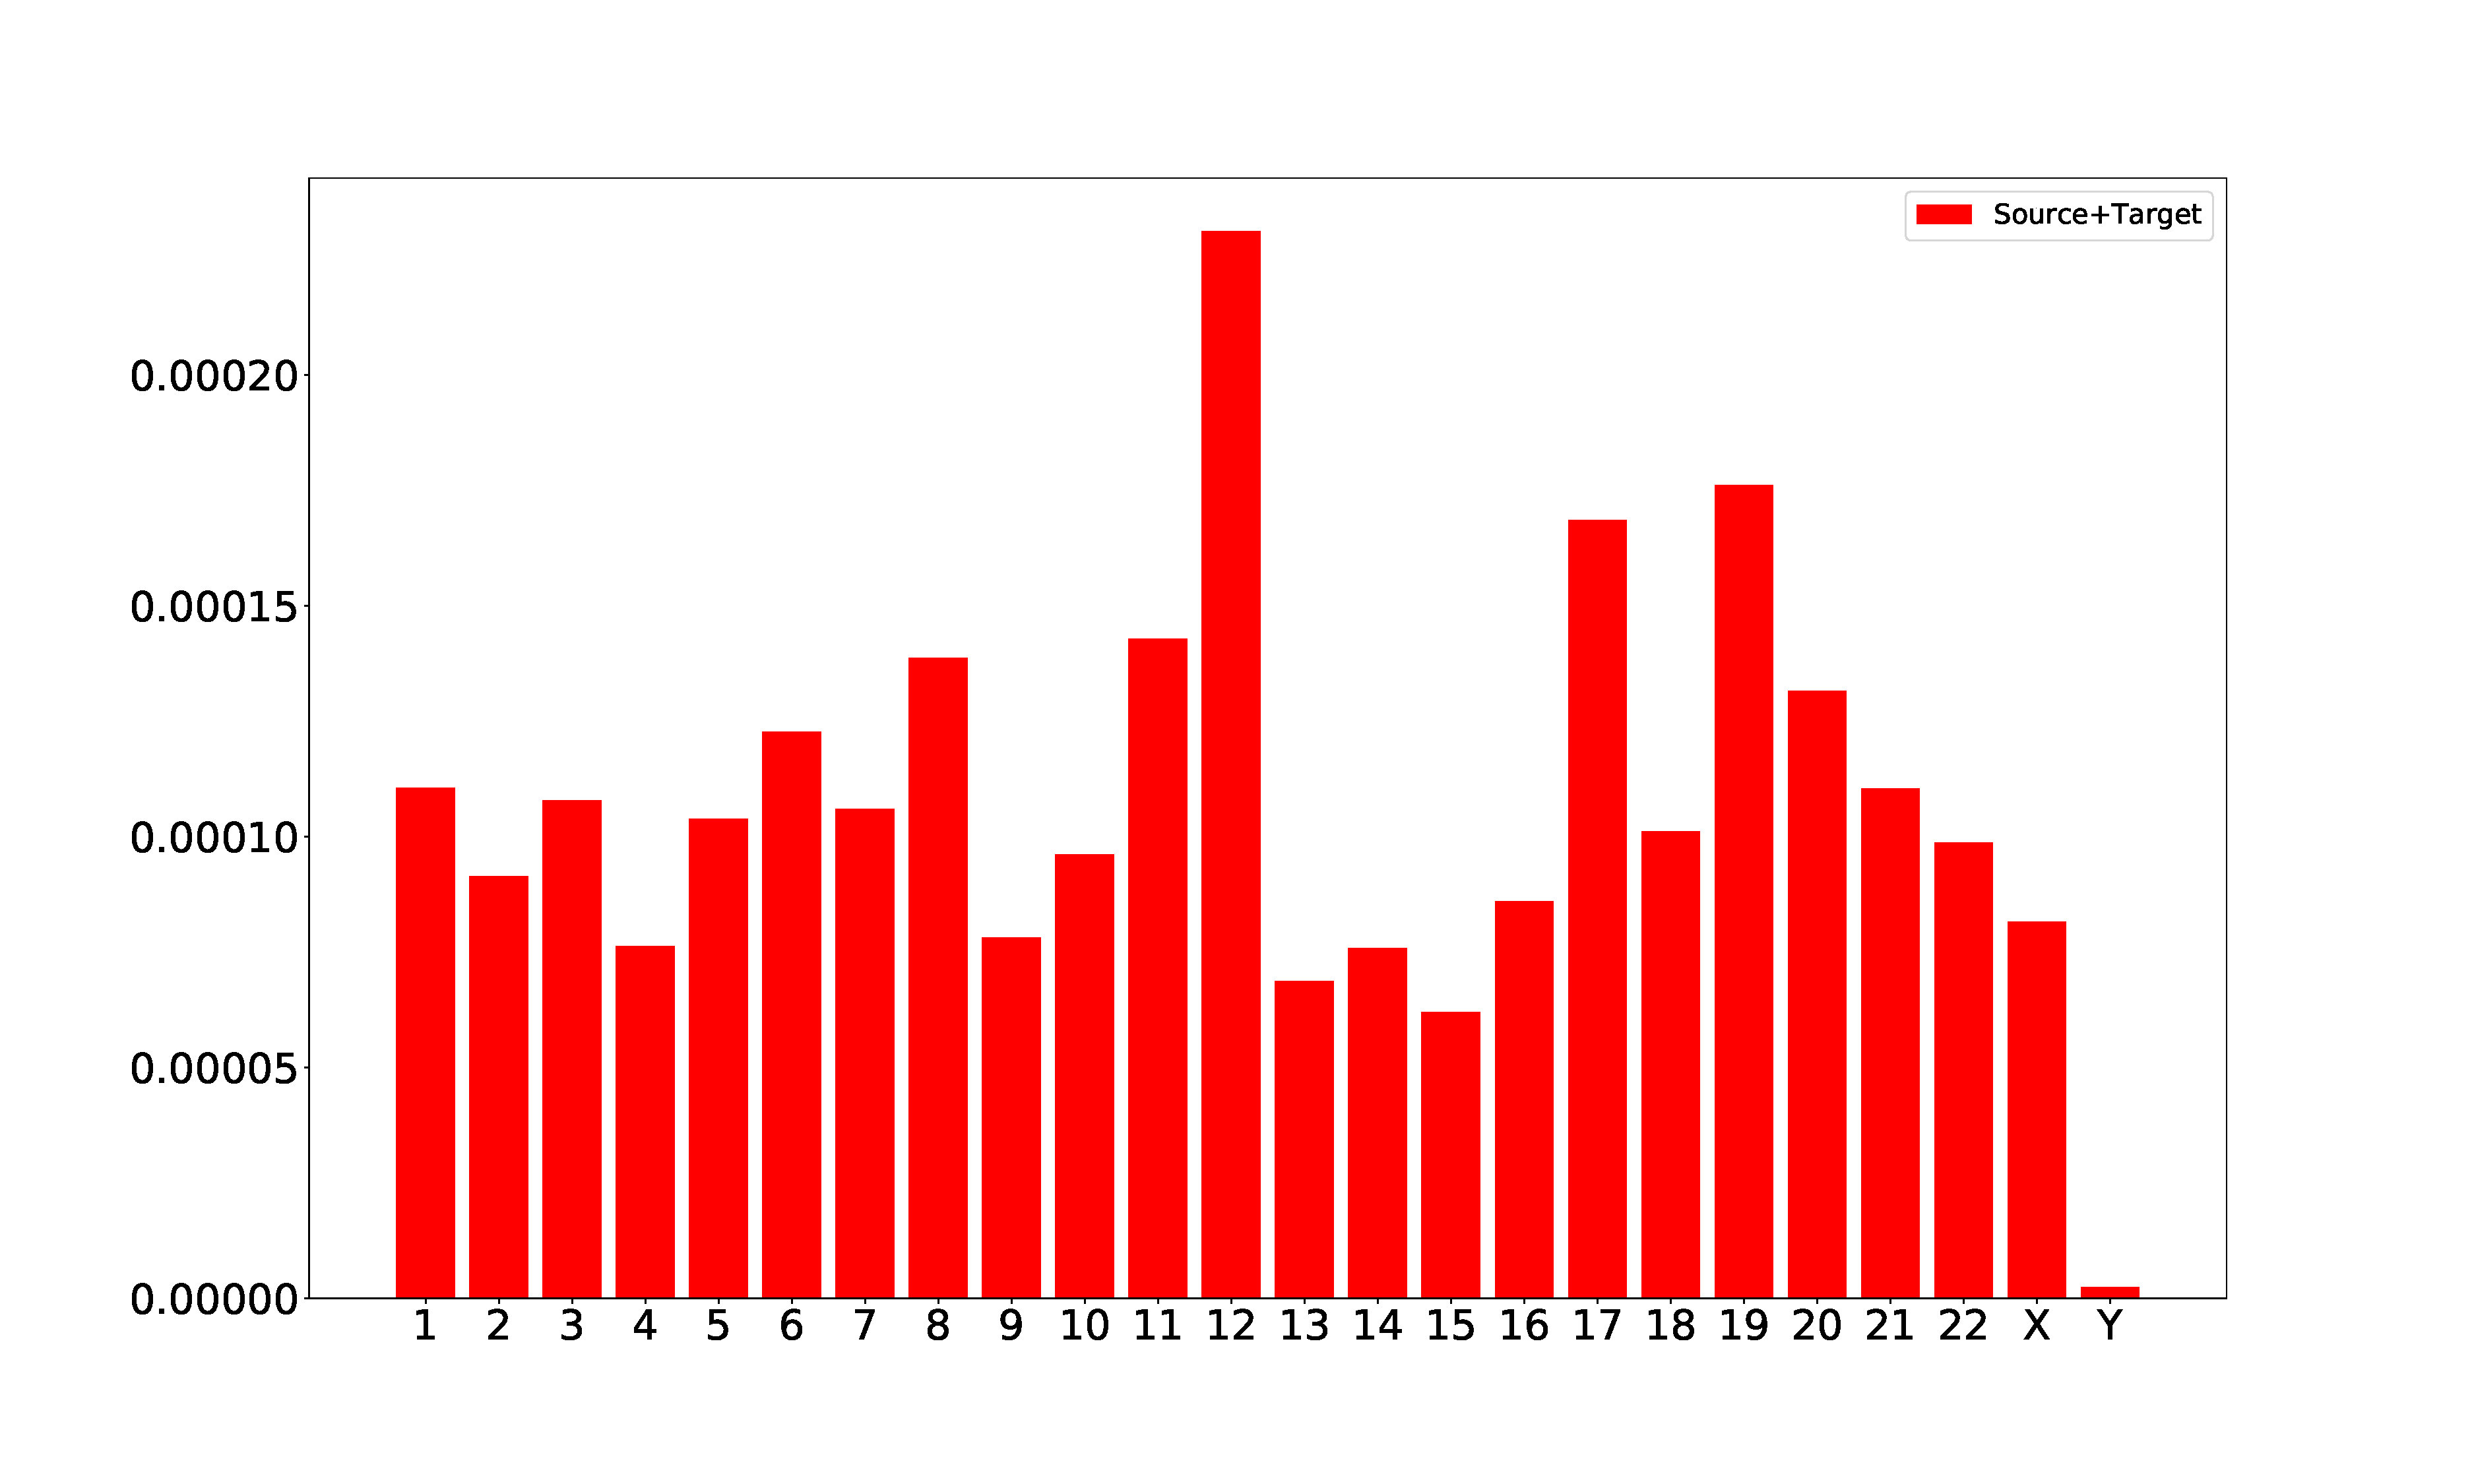
\includegraphics[scale=0.2]{figures/All_Break_distribution_normalized.pdf}
\caption{Distribution of breaks per chromosome. All brake types are aggregated. Values normalized by chromosome length}
\end{figure}

\subsection*{Distribution of breaks by type, unnormalized}

Next we plot the distribution of breaks by break type (h2hINV, DEL, t2tINV, DUP, TRA), unnormalized

\begin{figure}[H]
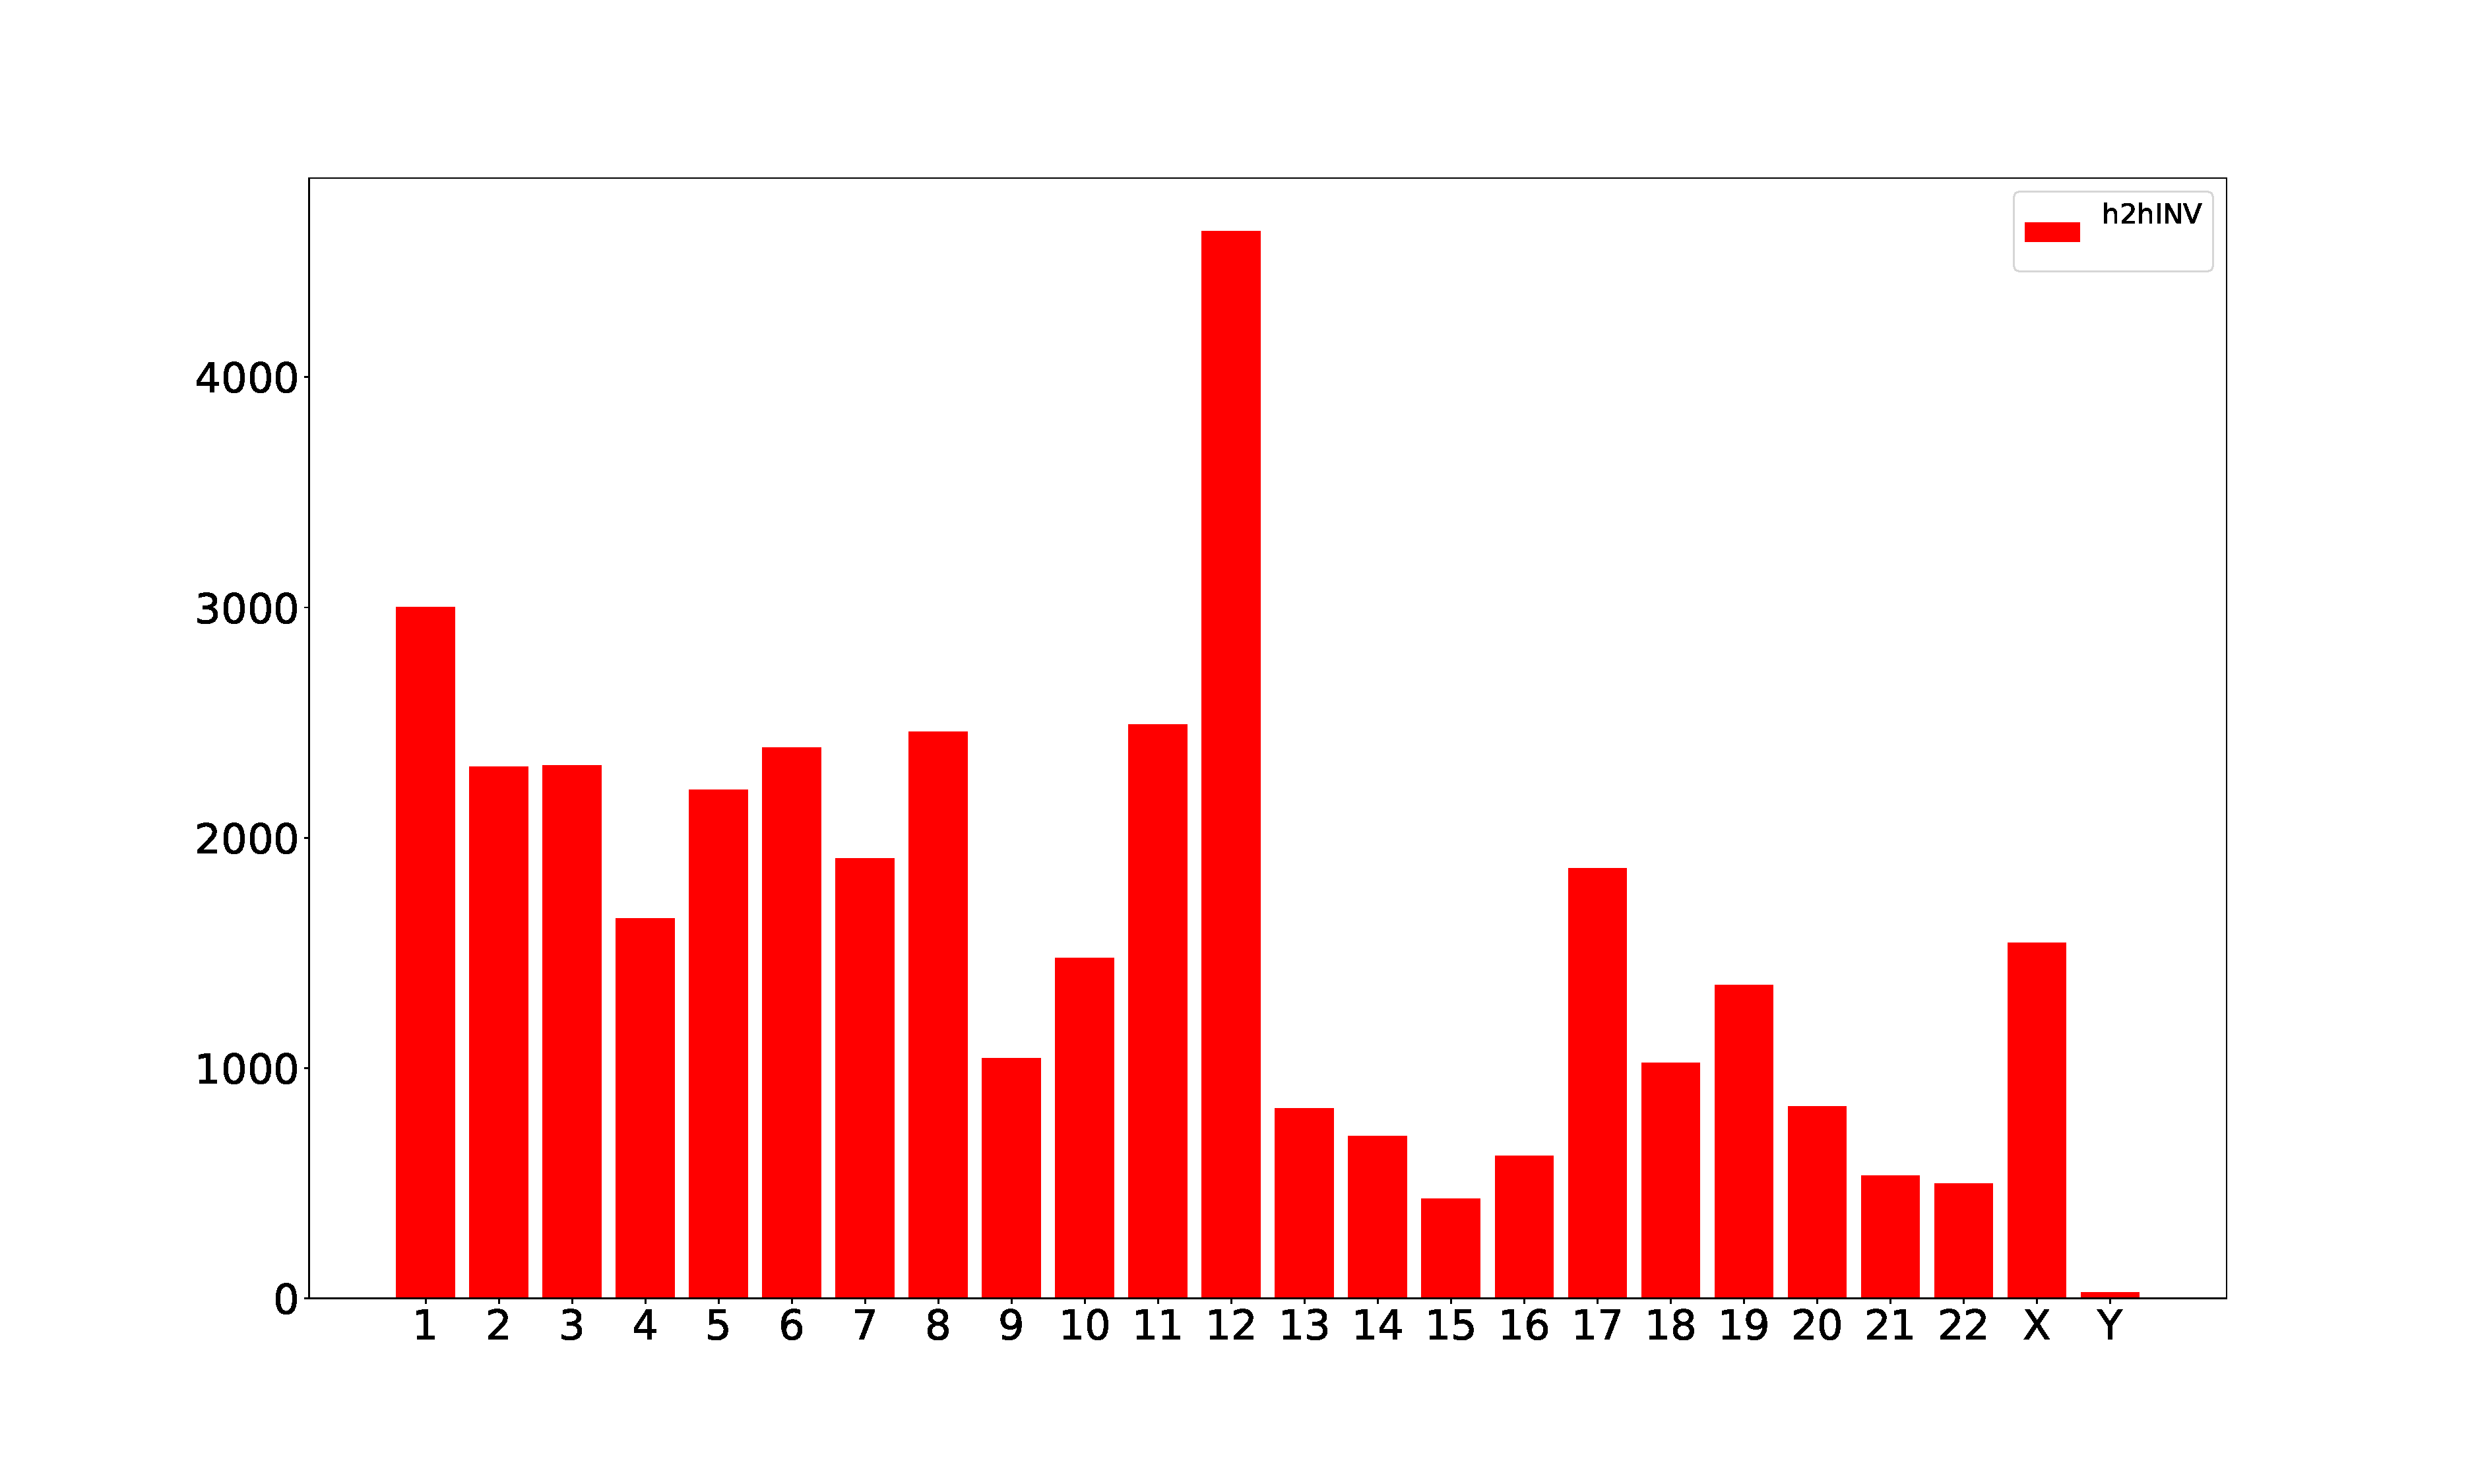
\includegraphics[scale=0.2]{figures/h2hINV_Break_distribution_unnormalized.pdf}
\caption{Distribution of h2hINV breaks per chromosome. Values unnormalized}
\end{figure}

\begin{figure}[H]
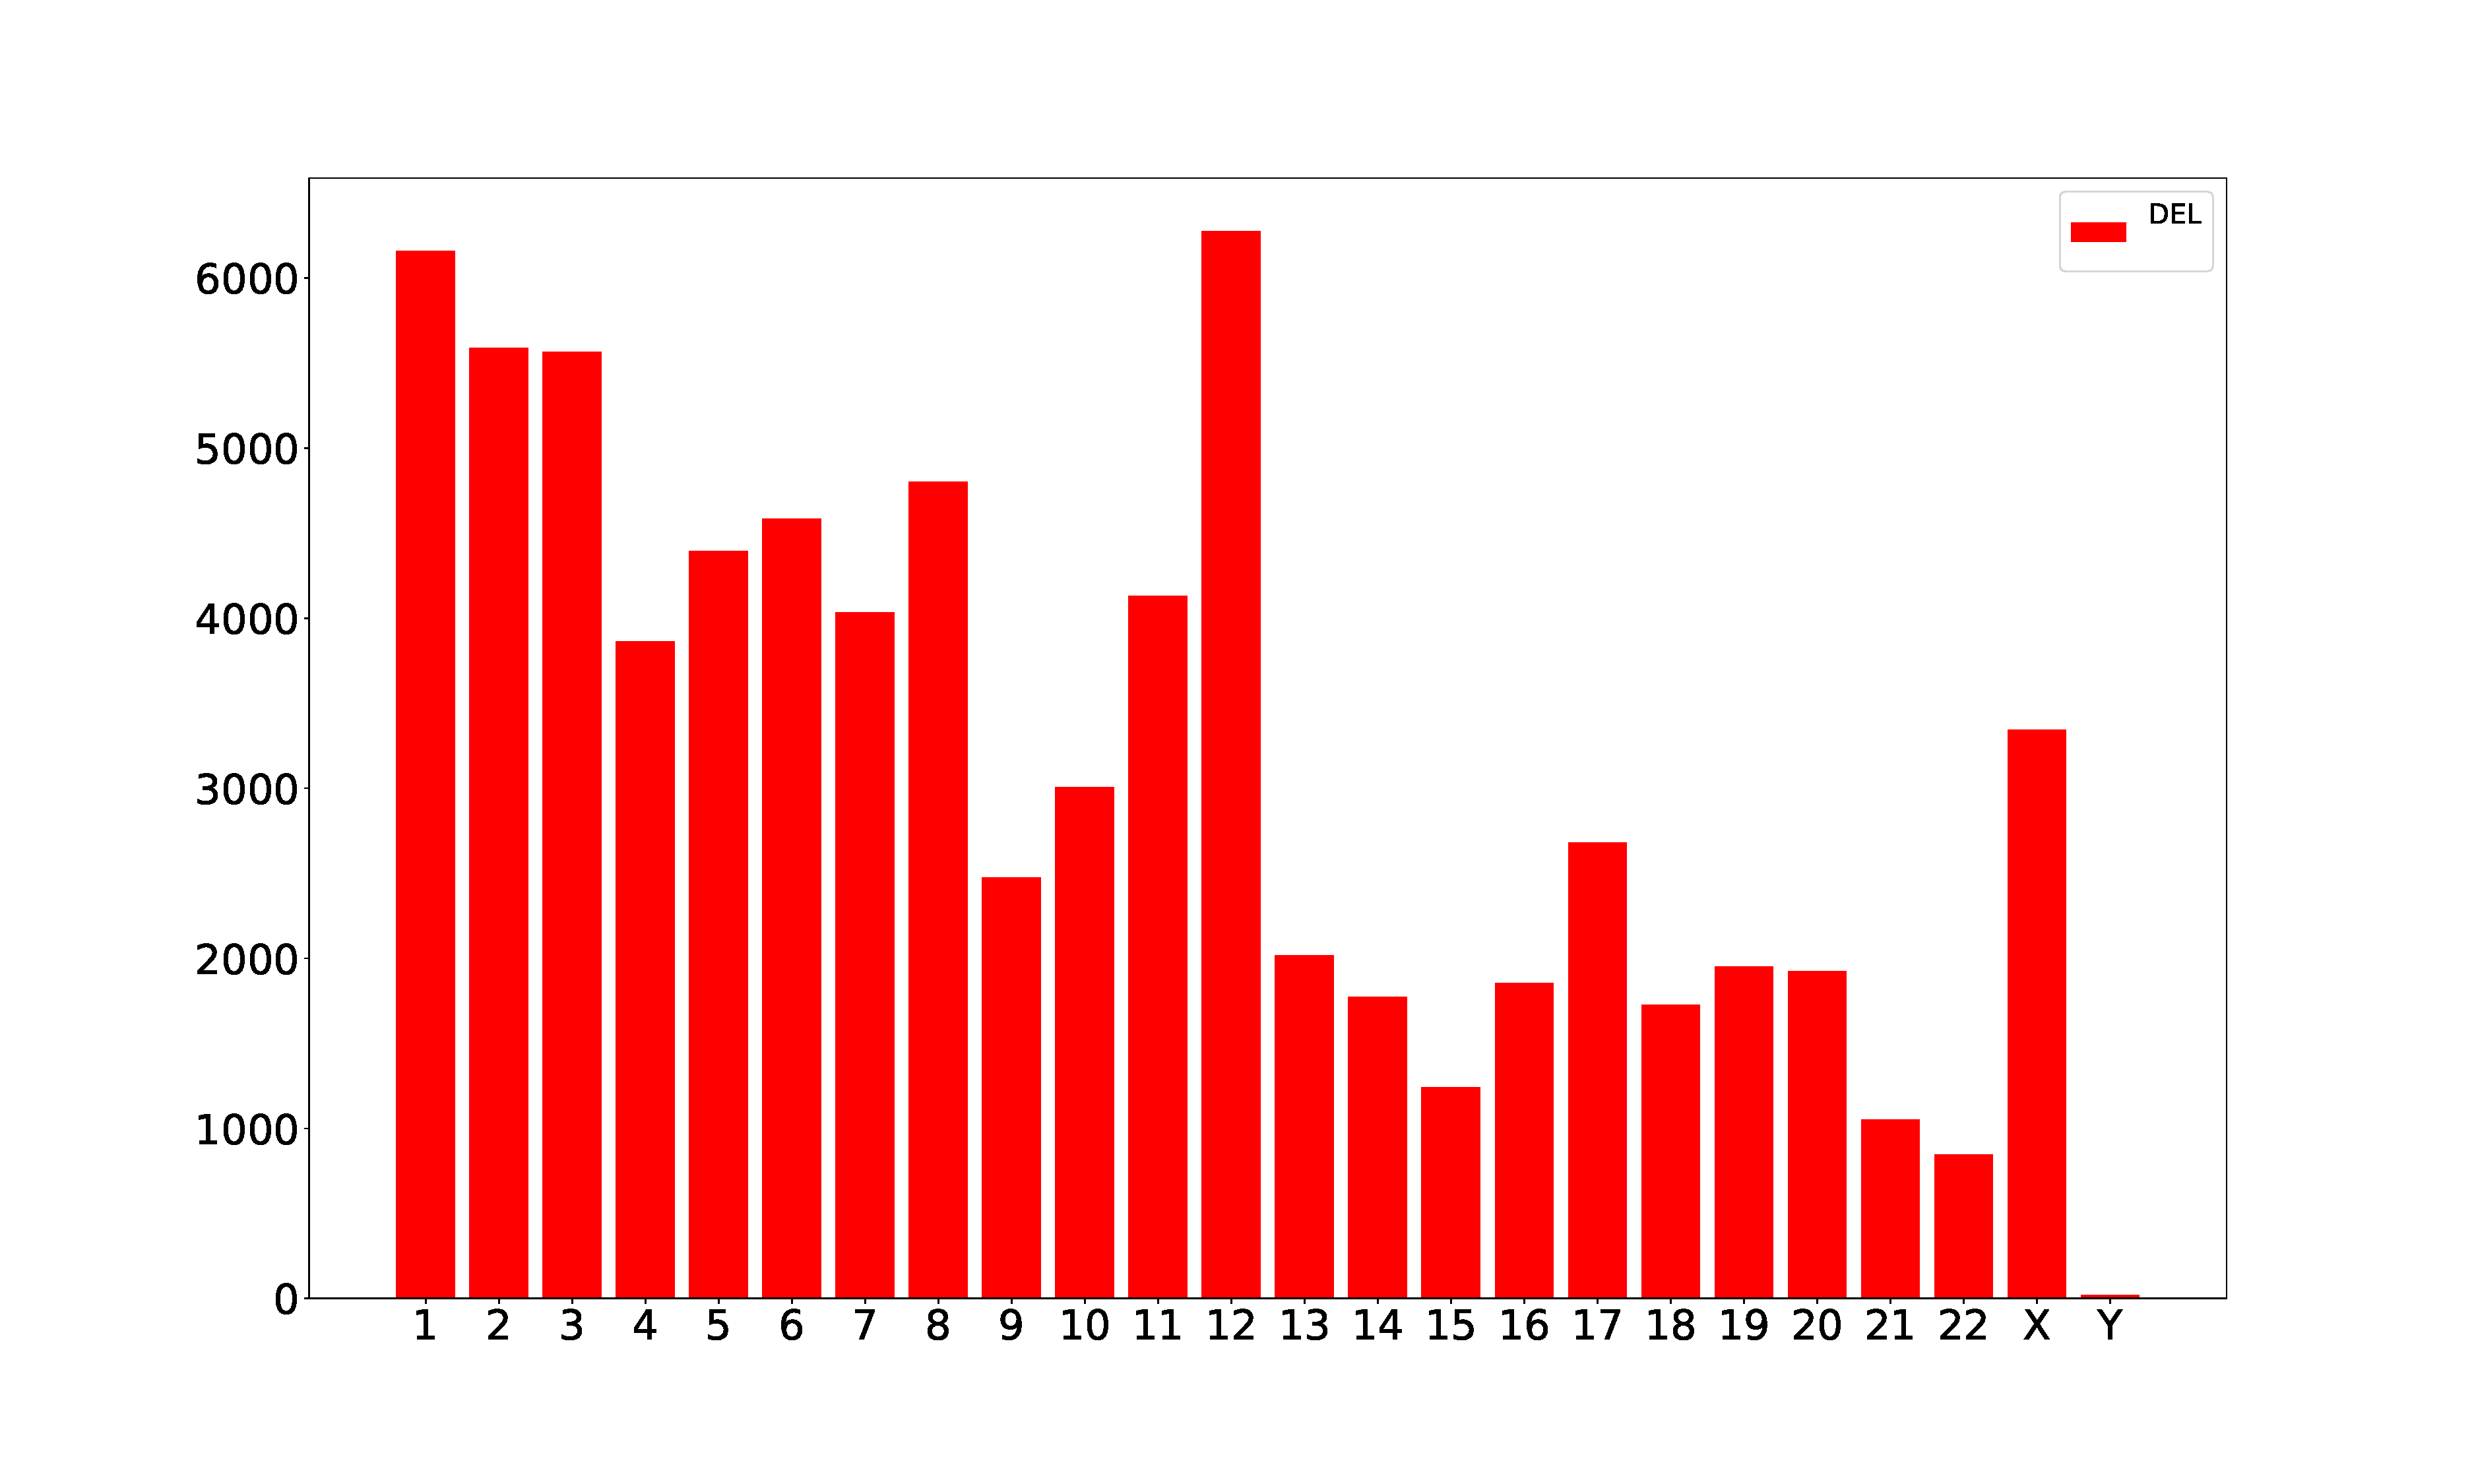
\includegraphics[scale=0.2]{figures/DEL_Break_distribution_unnormalized.pdf}
\caption{Distribution of DEL breaks per chromosome. Values unnormalized}
\end{figure}

\begin{figure}[H]
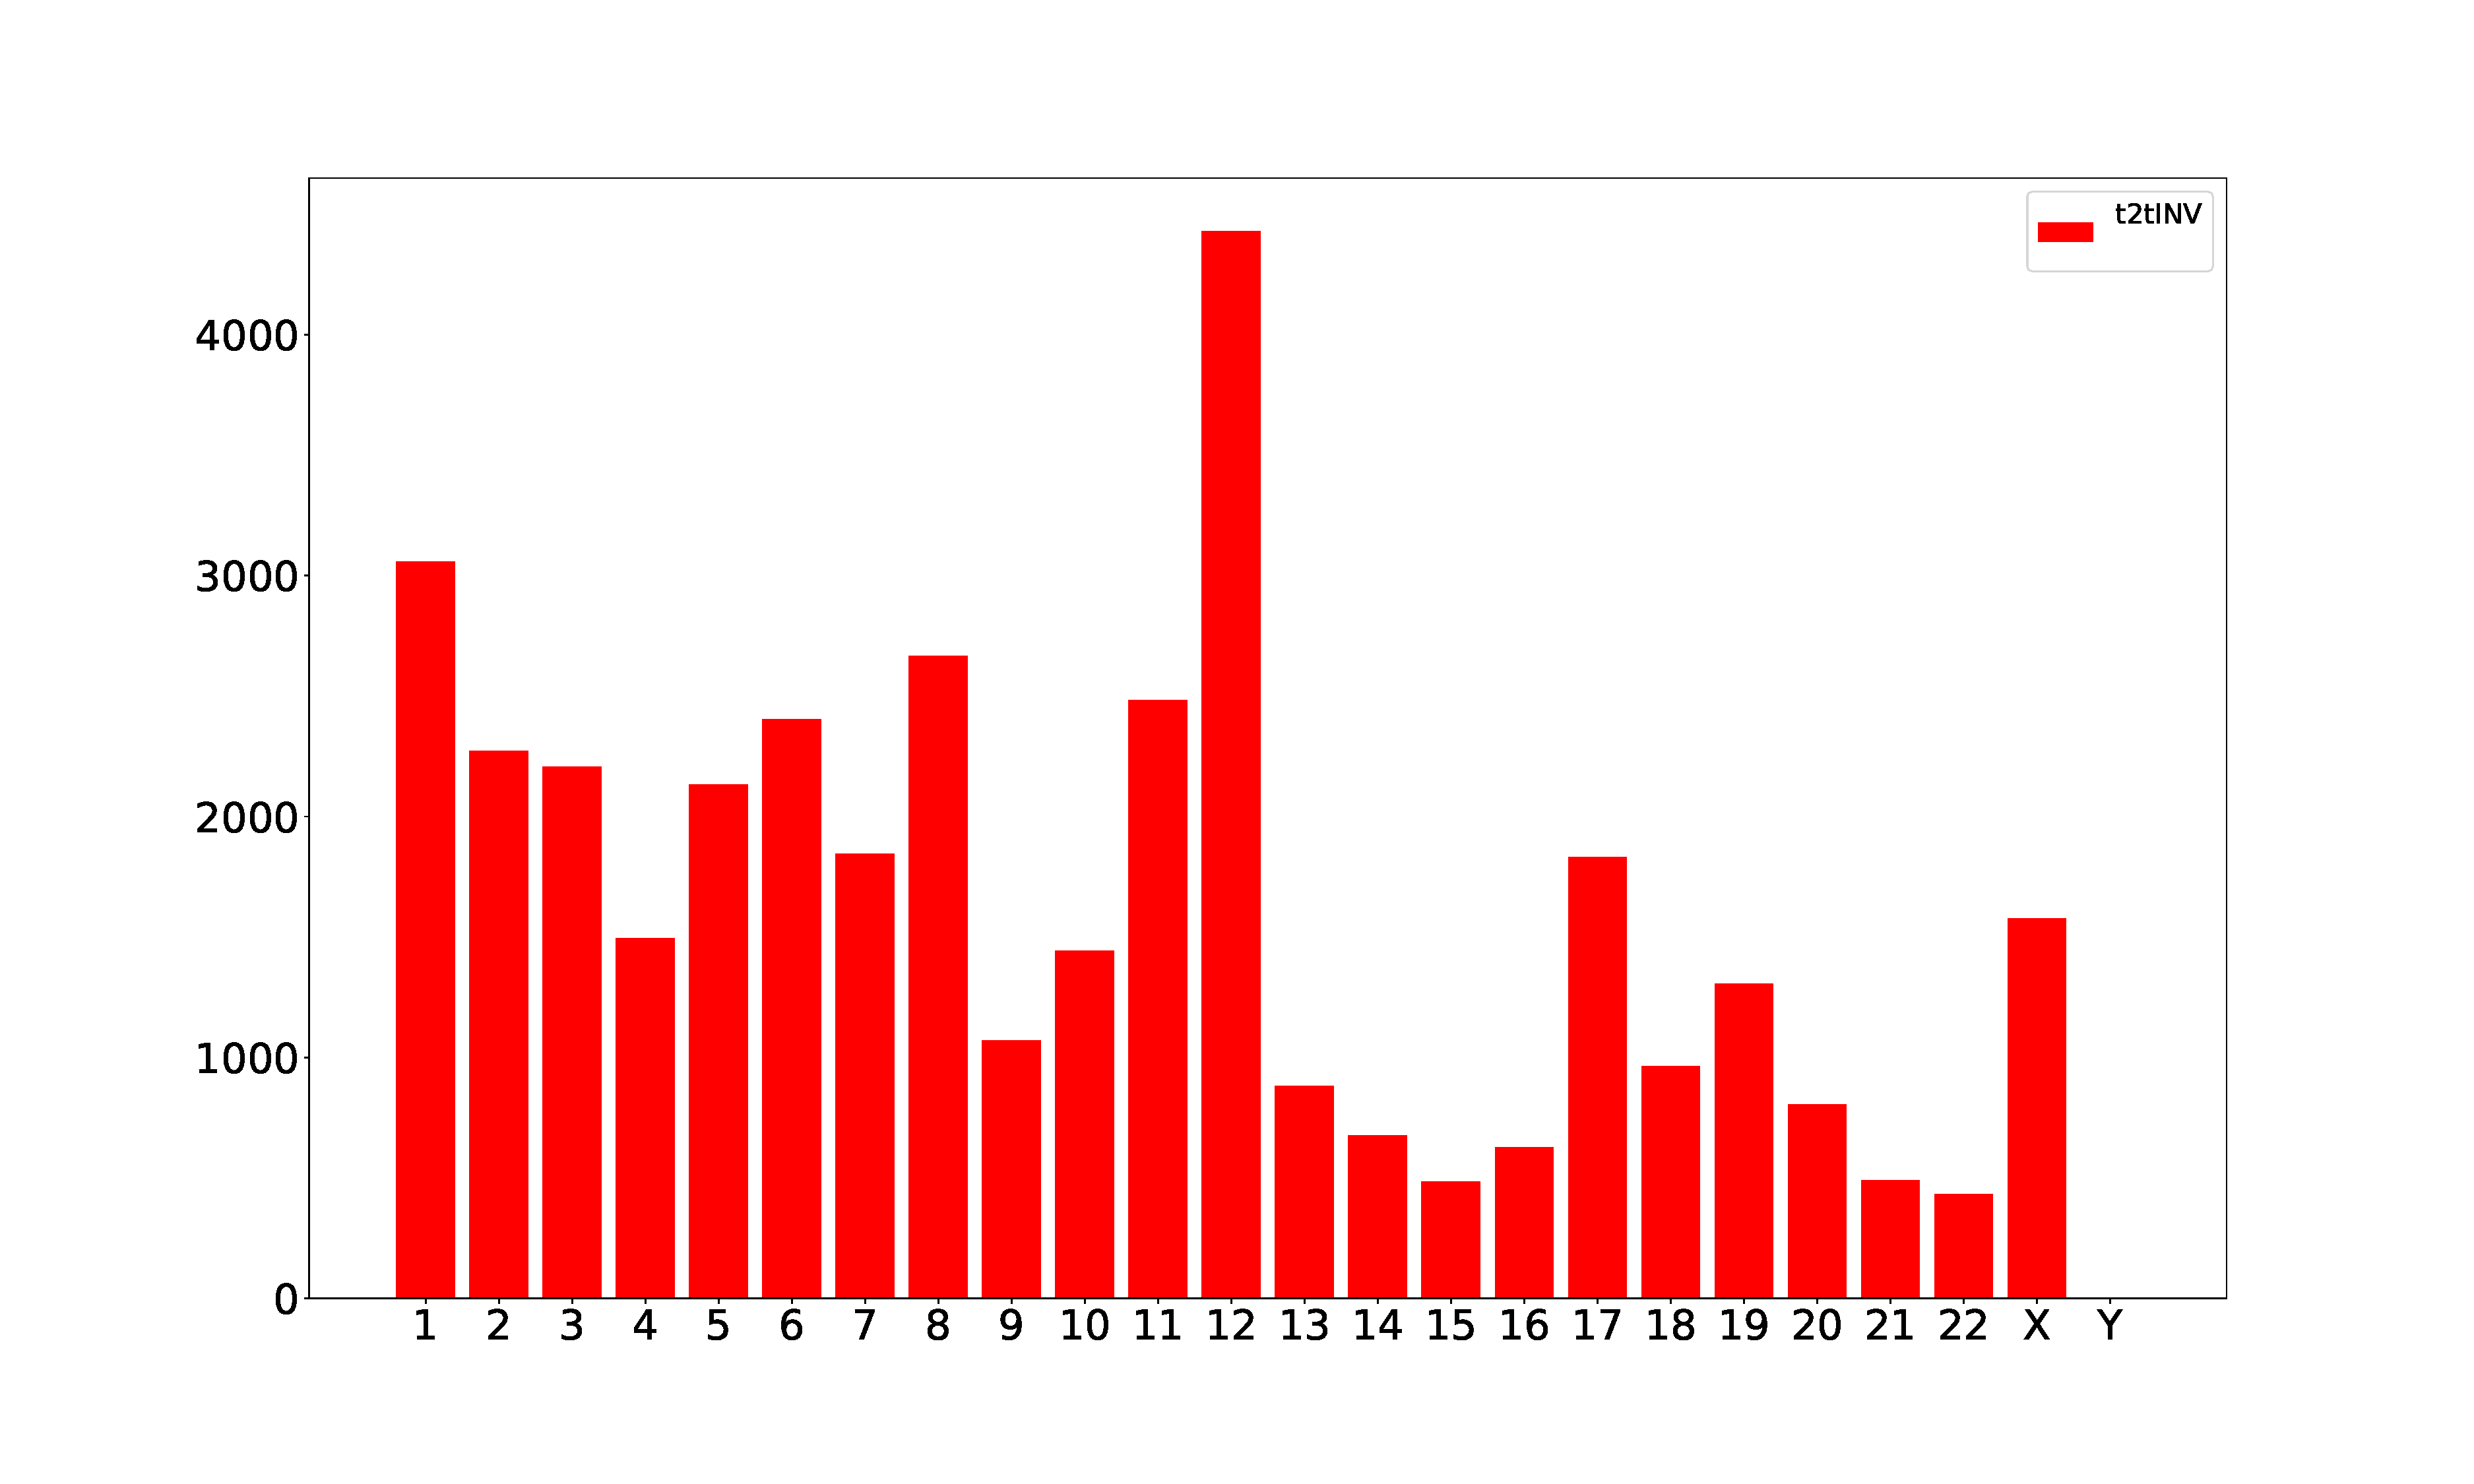
\includegraphics[scale=0.2]{figures/t2tINV_Break_distribution_unnormalized.pdf}
\caption{Distribution of t2tINV breaks per chromosome. Values unnormalized}
\end{figure}

\begin{figure}[H]
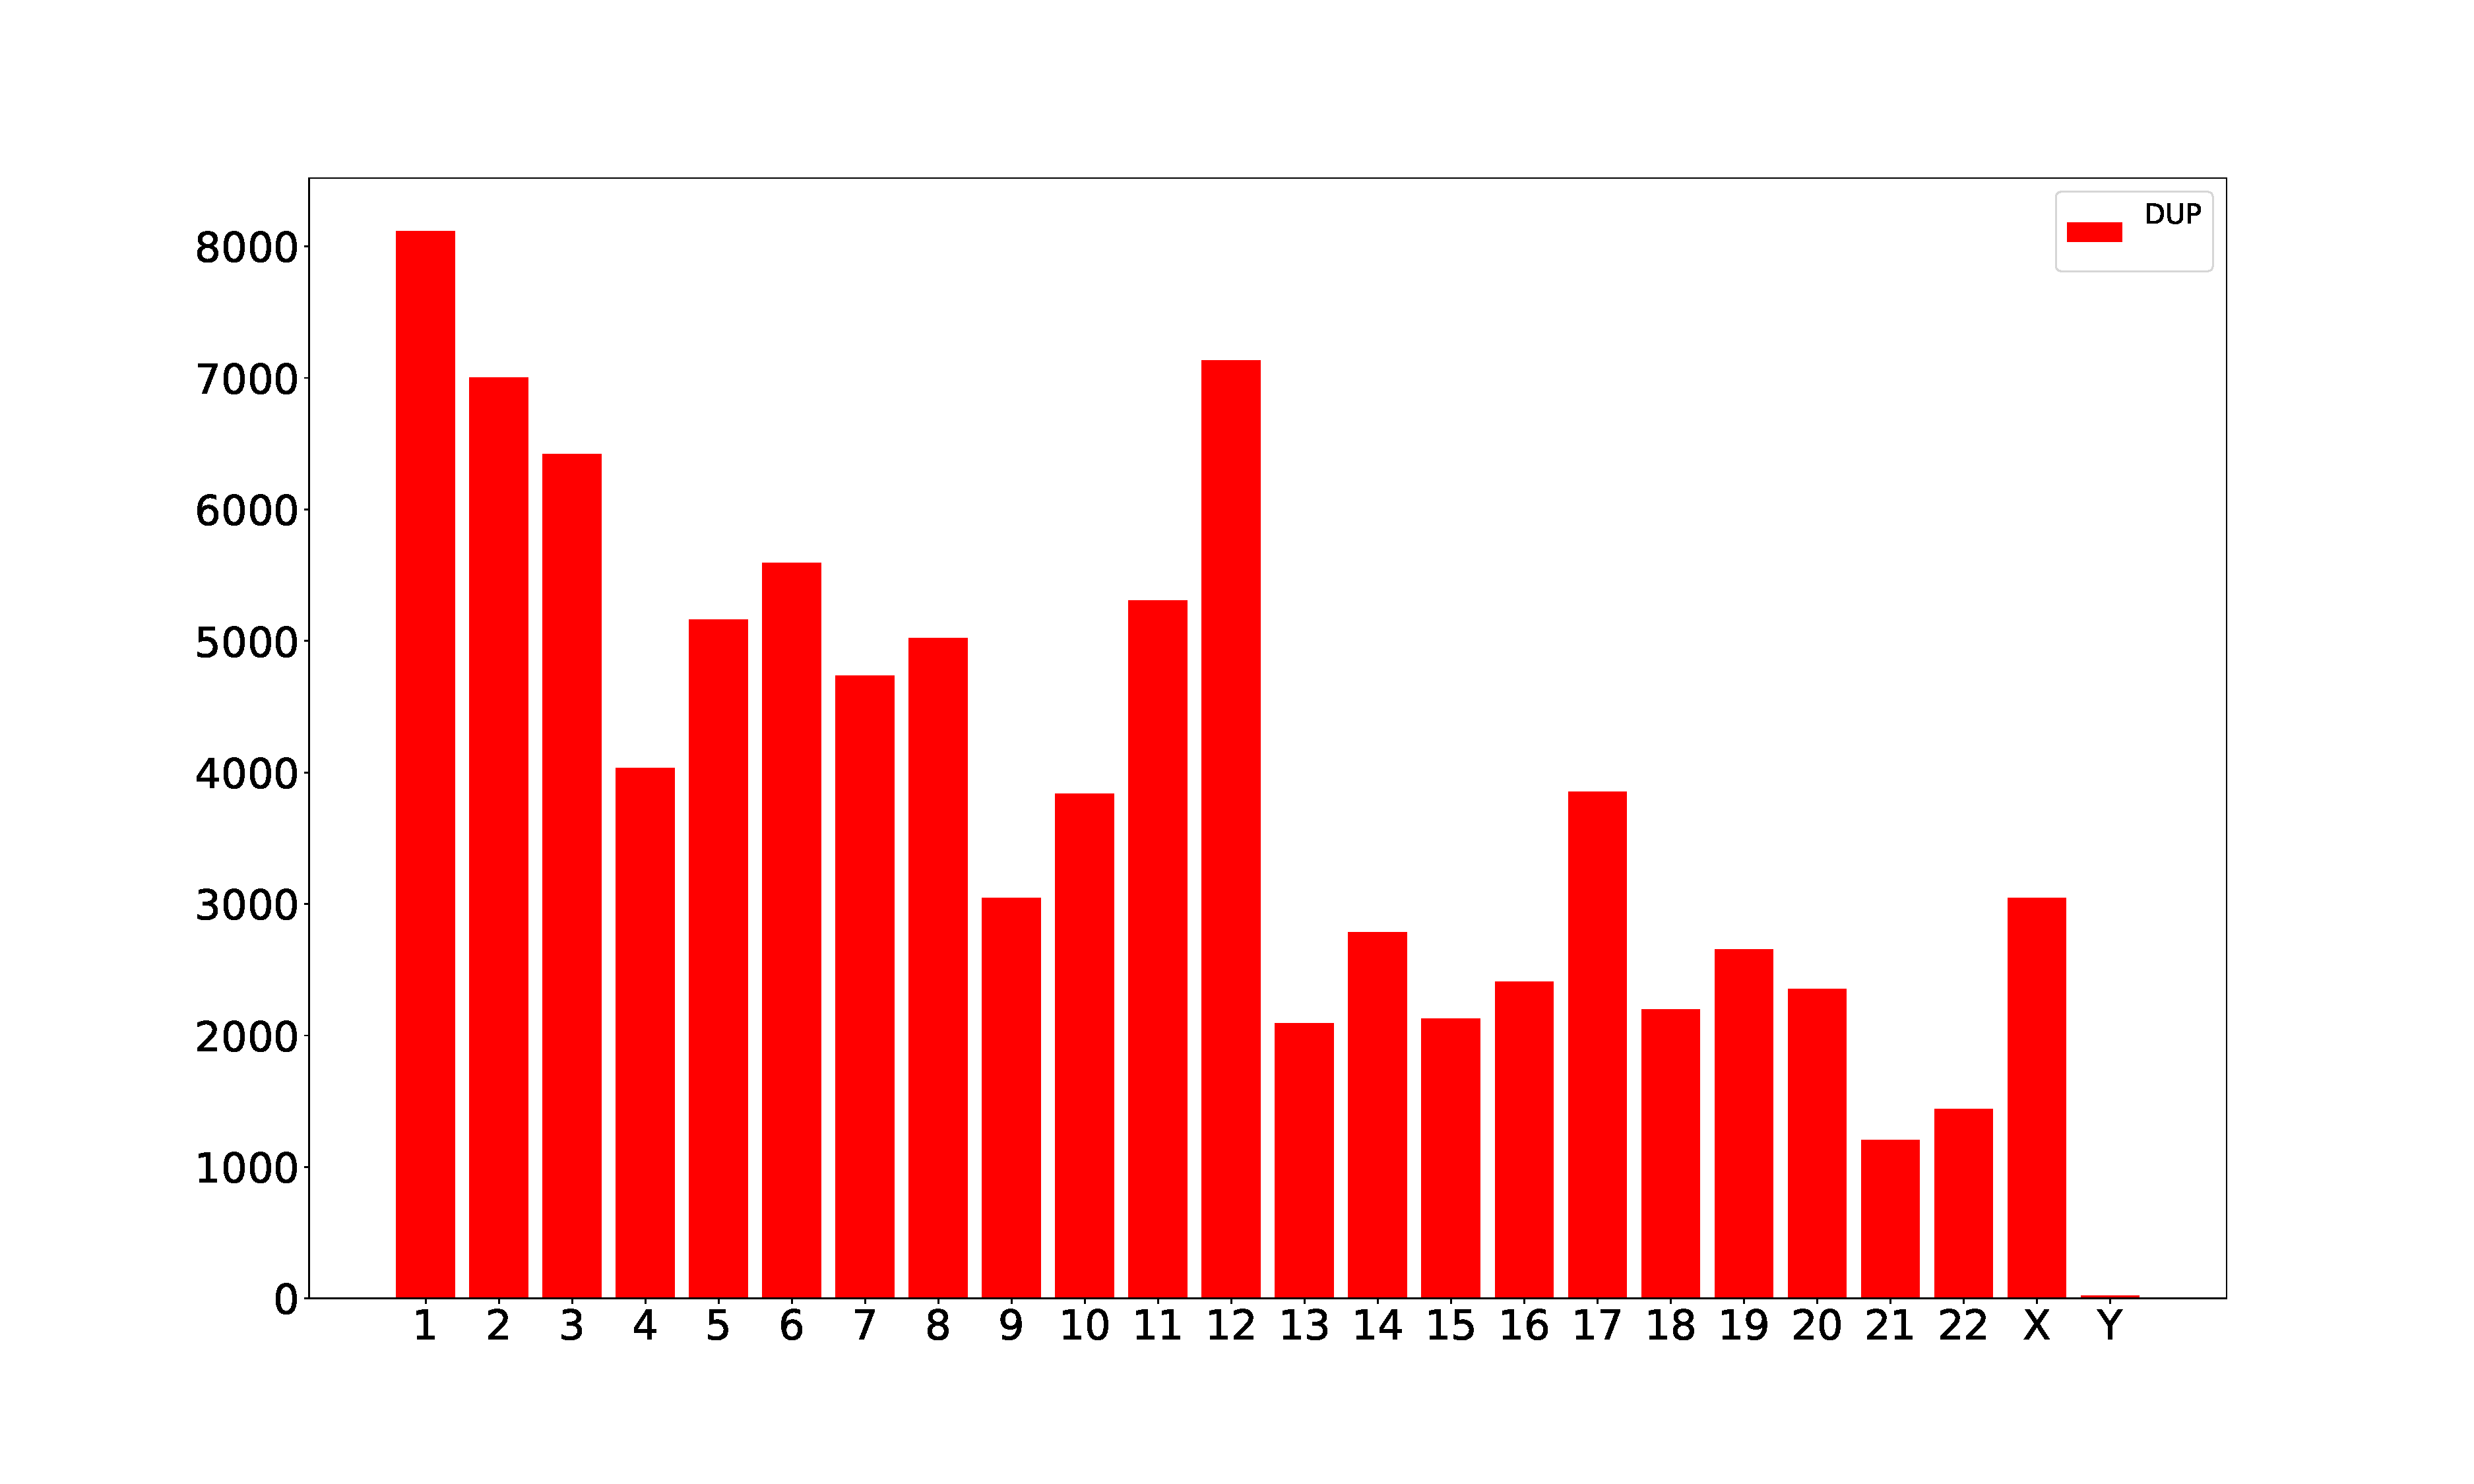
\includegraphics[scale=0.2]{figures/DUP_Break_distribution_unnormalized.pdf}
\caption{Distribution of DUP breaks per chromosome. Values unnormalized}
\end{figure}

\begin{figure}[H]
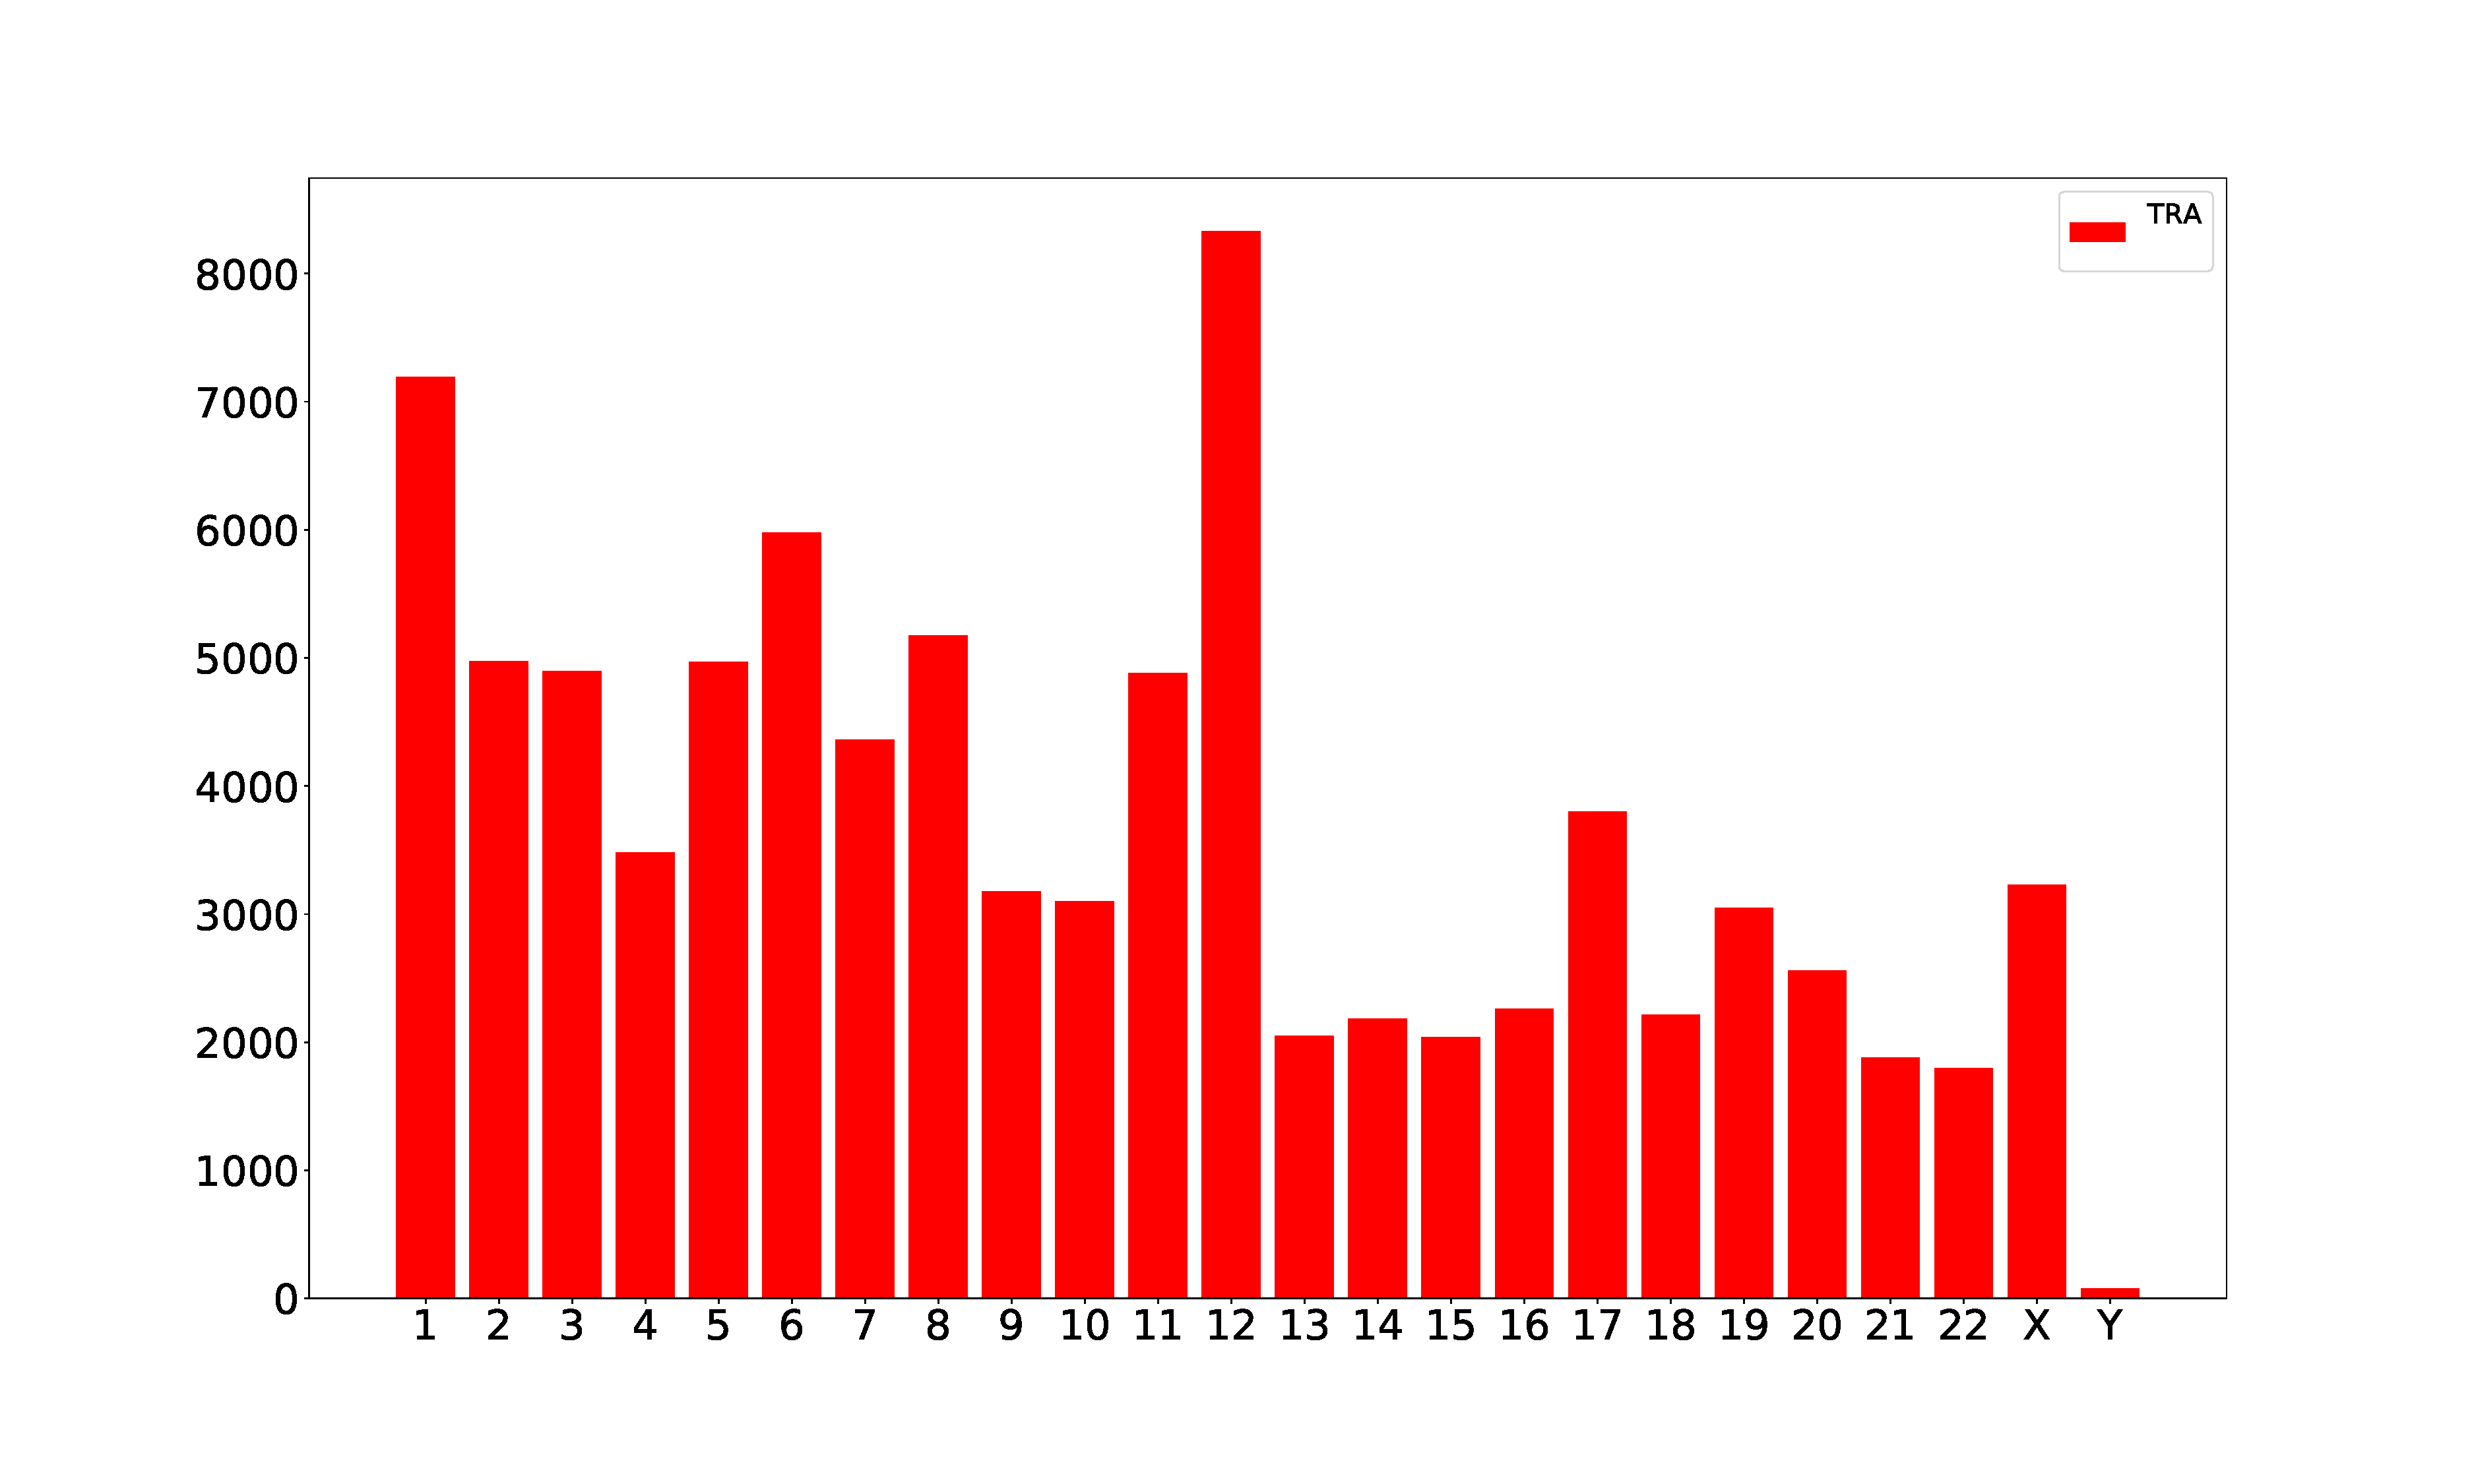
\includegraphics[scale=0.2]{figures/TRA_Break_distribution_unnormalized.pdf}
\caption{Distribution of TRA breaks per chromosome. Values unnormalized}
\end{figure}

\pagebreak

\subsection*{Distribution of breaks by type, normalized}

Next we plot the distribution of breaks by break type (h2hINV, DEL, t2tINV, DUP, TRA), normalized by chromosome length

\begin{figure}[H]
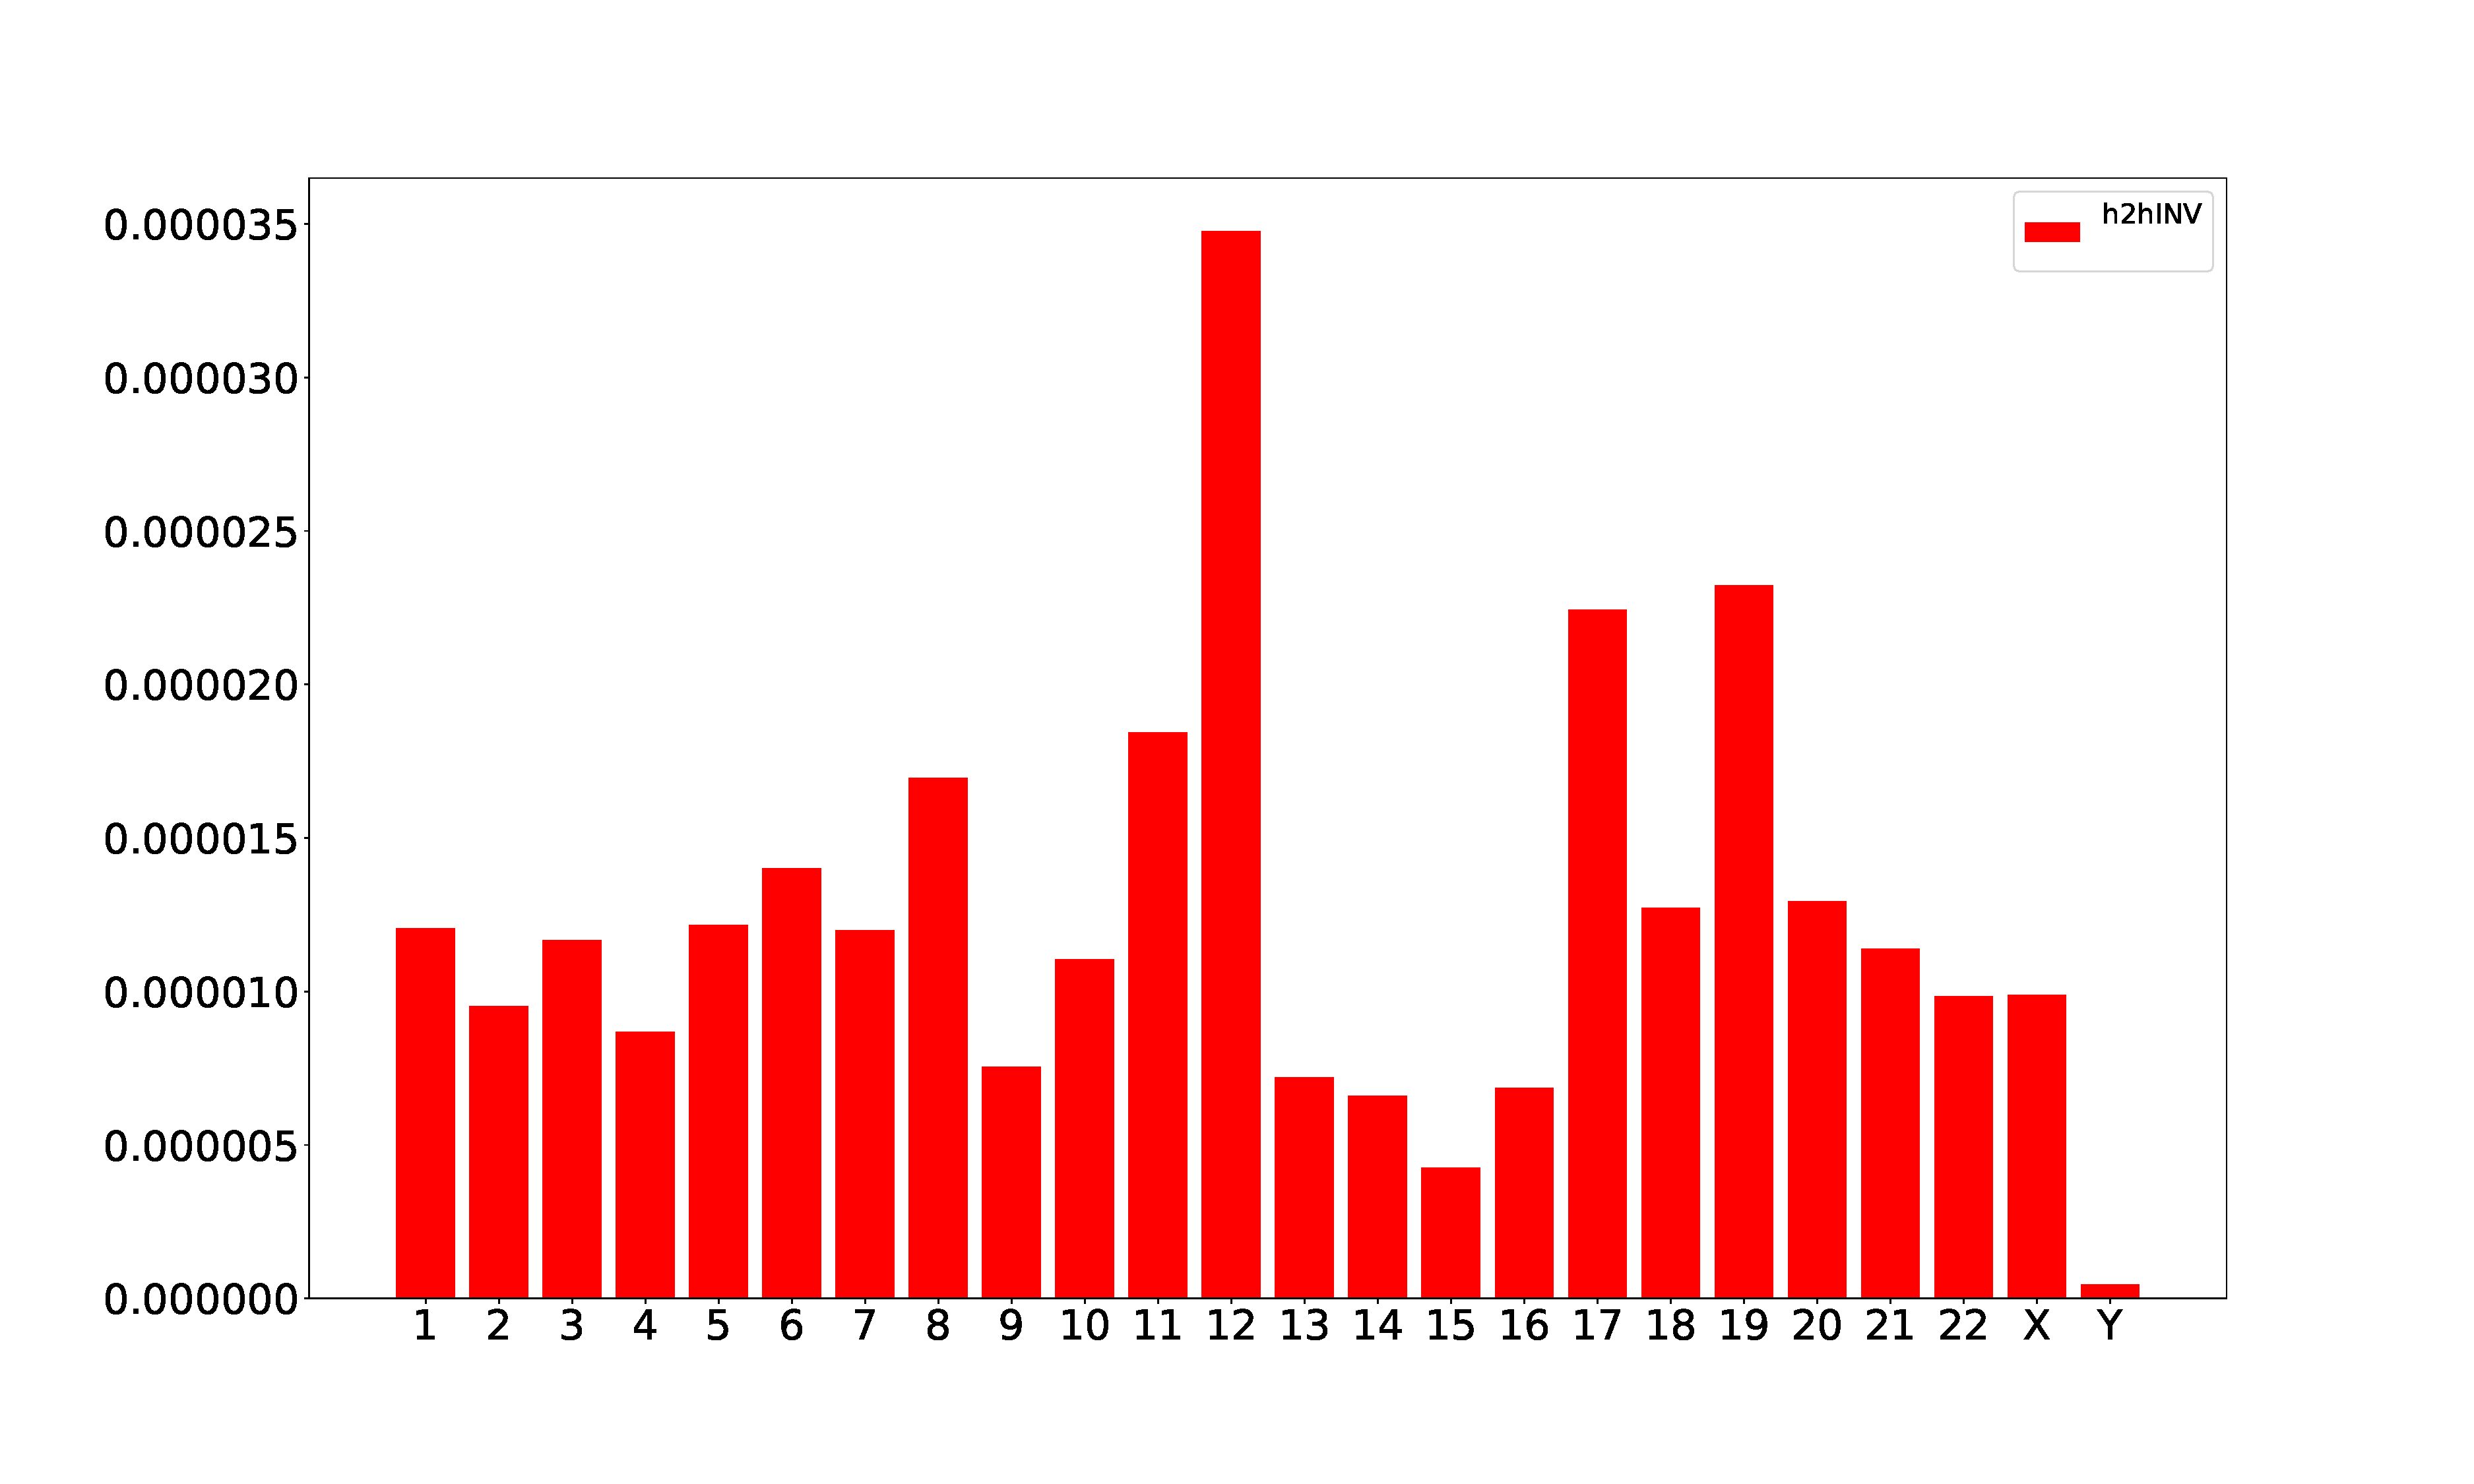
\includegraphics[scale=0.2]{figures/h2hINV_Break_distribution_normalized.pdf}
\caption{Distribution of h2hINV breaks per chromosome. Values normalized by chromosome length}
\end{figure}

\begin{figure}[H]
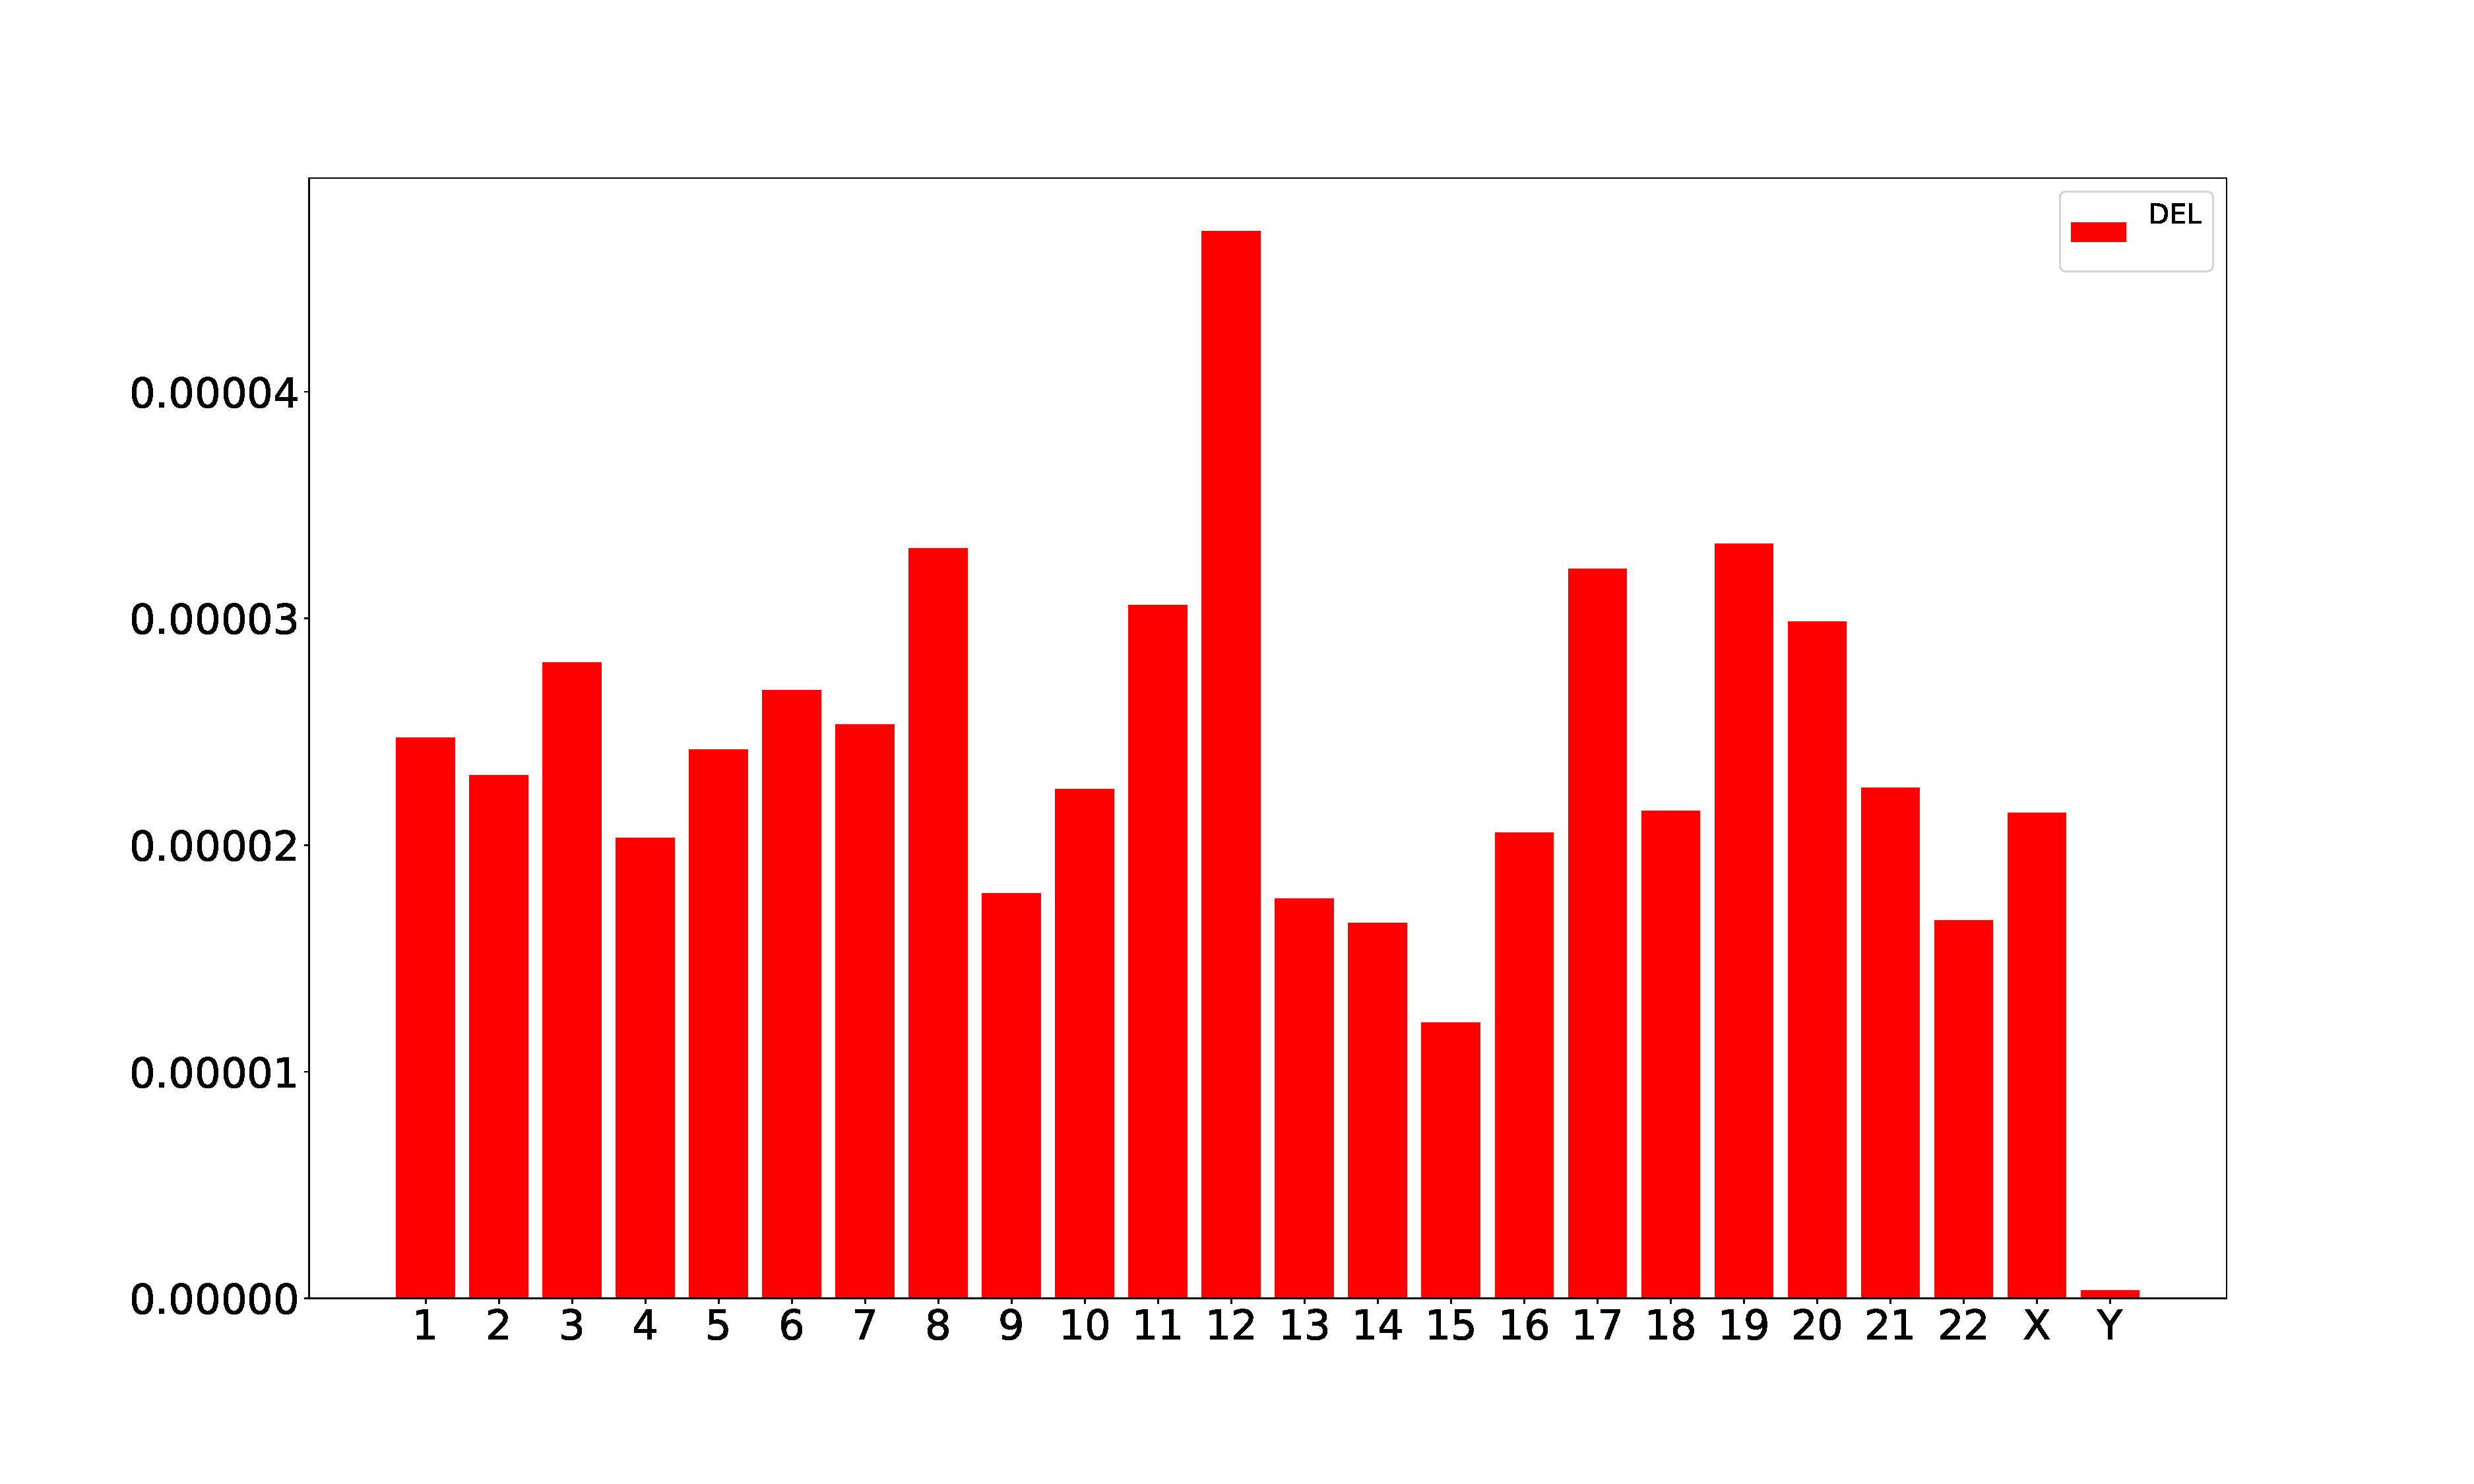
\includegraphics[scale=0.2]{figures/DEL_Break_distribution_normalized.pdf}
\caption{Distribution of DEL breaks per chromosome. Values normalized by chromosome length}
\end{figure}

\begin{figure}[H]
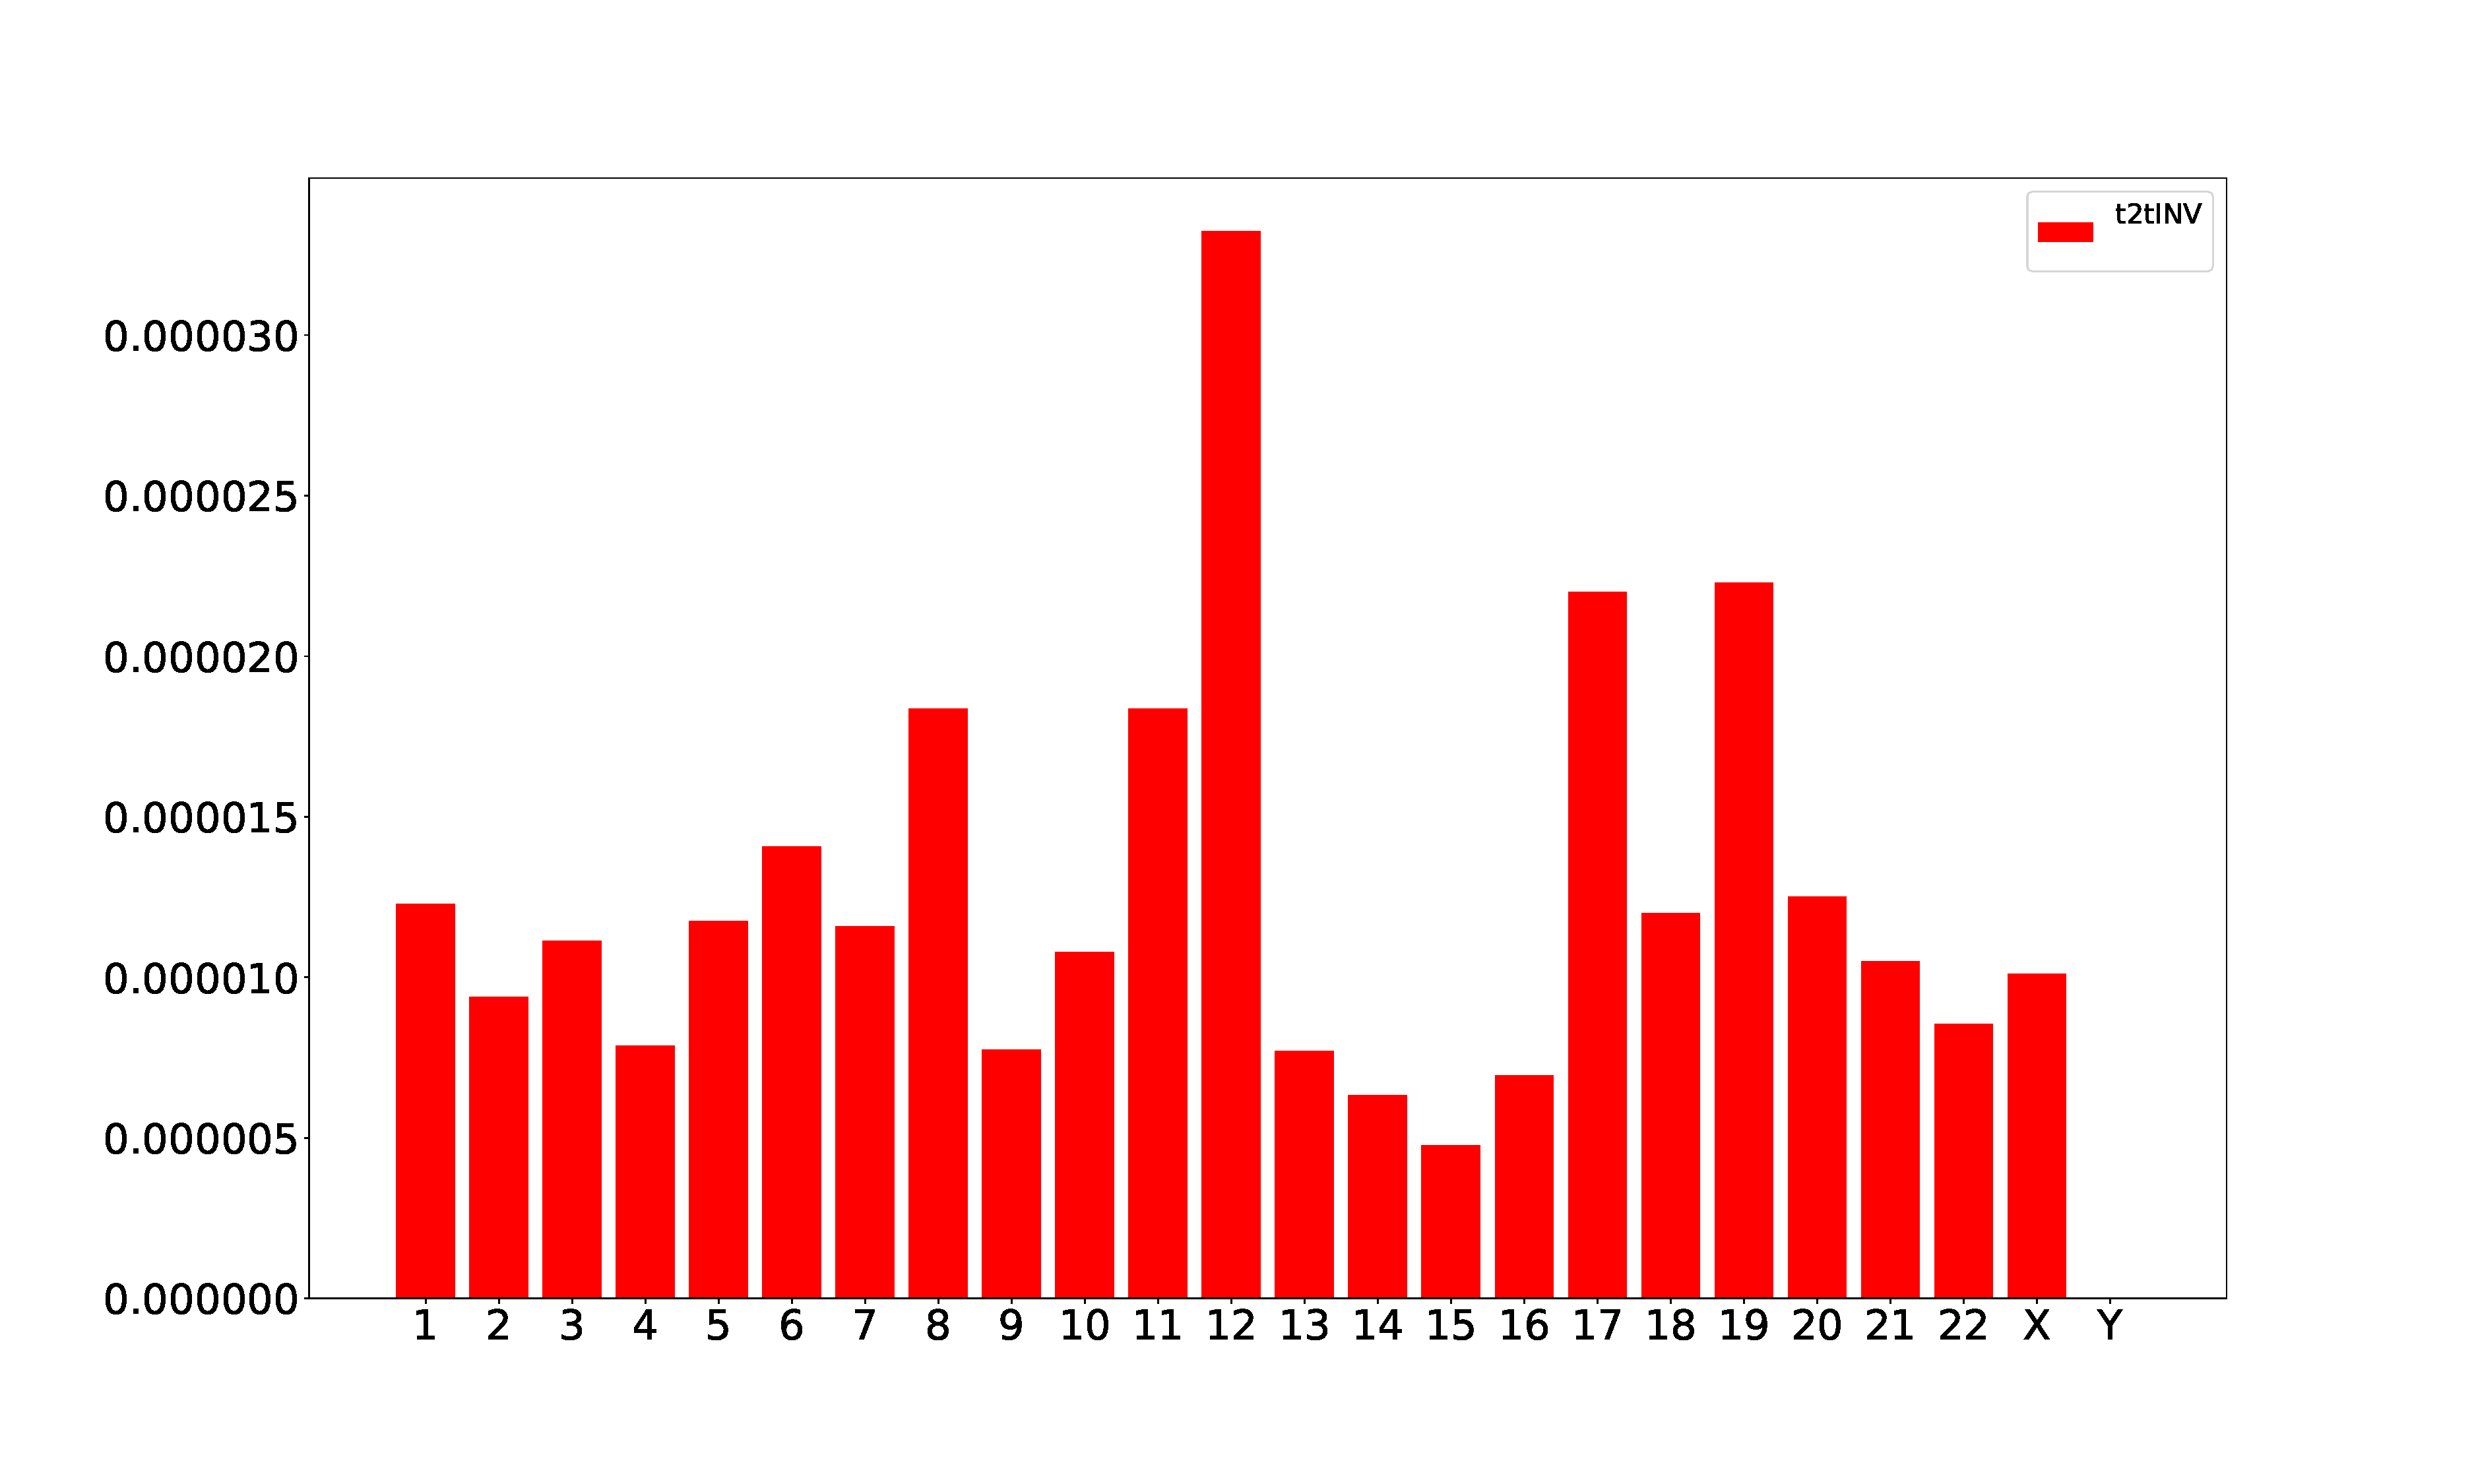
\includegraphics[scale=0.2]{figures/t2tINV_Break_distribution_normalized.pdf}
\caption{Distribution of t2tINV breaks per chromosome. Values normalized by chromosome length}
\end{figure}

\begin{figure}[H]
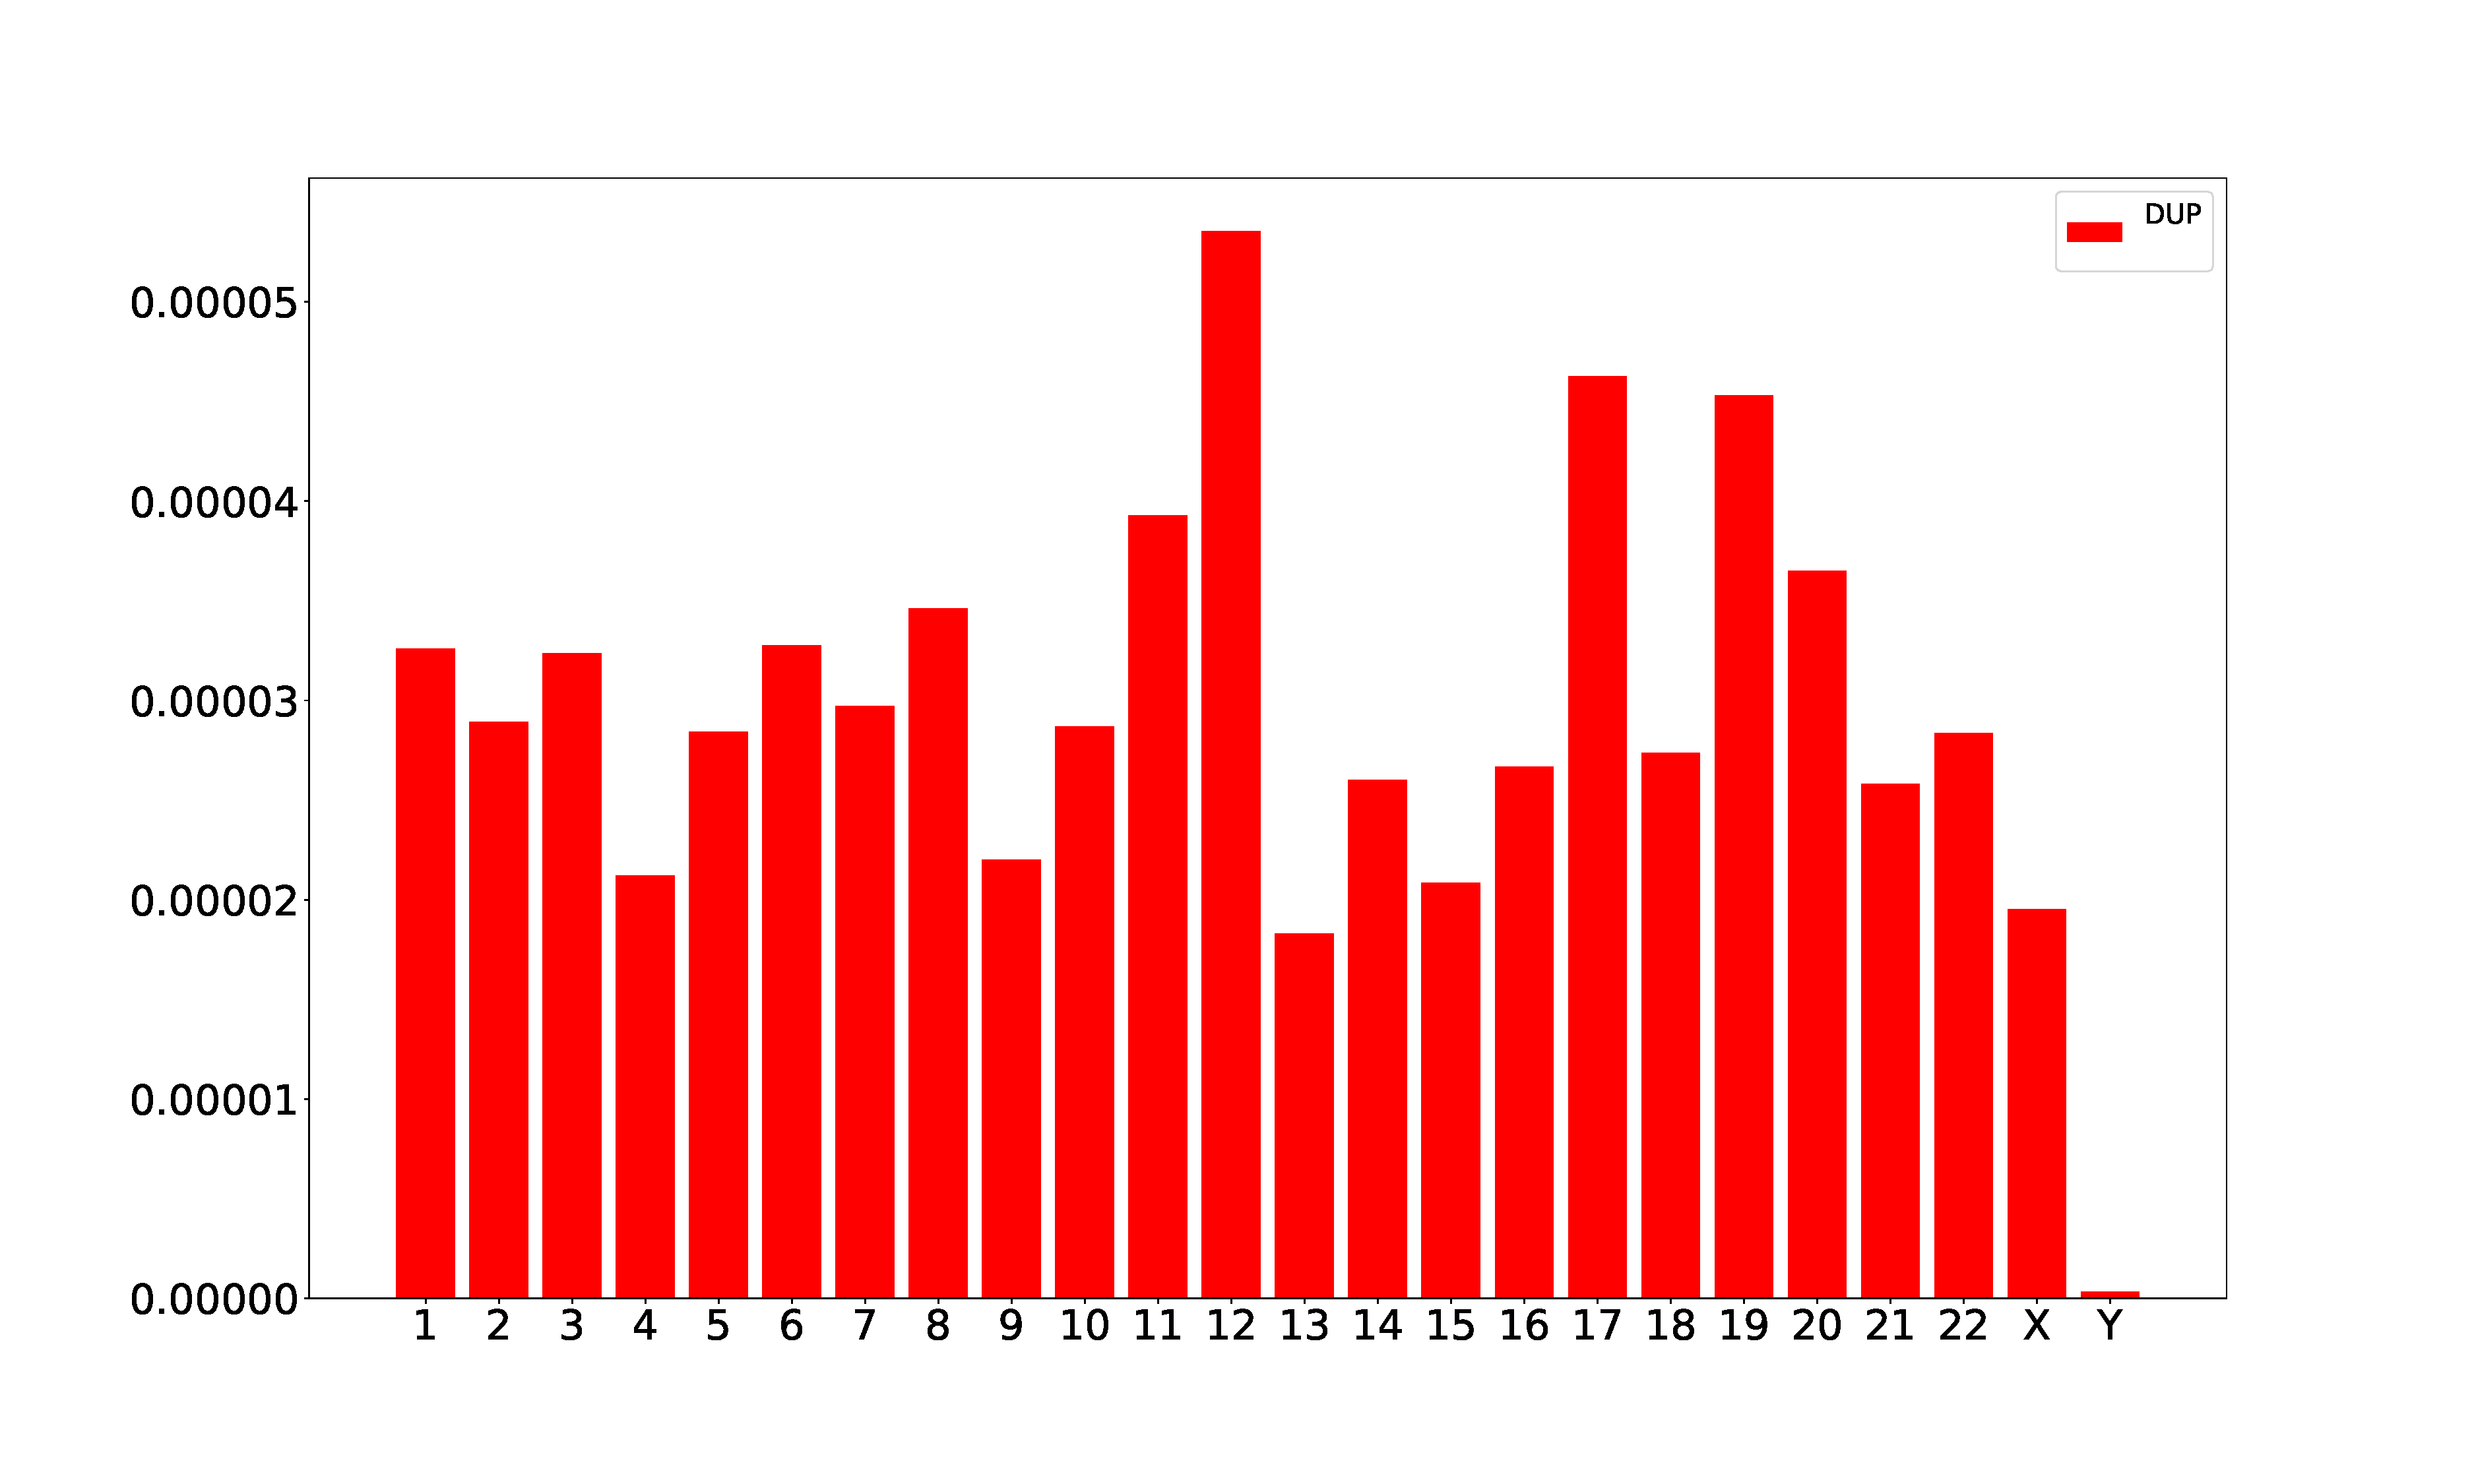
\includegraphics[scale=0.2]{figures/DUP_Break_distribution_normalized.pdf}
\caption{Distribution of DUP breaks per chromosome. Values normalized by chromosome length}
\end{figure}

\begin{figure}[H]
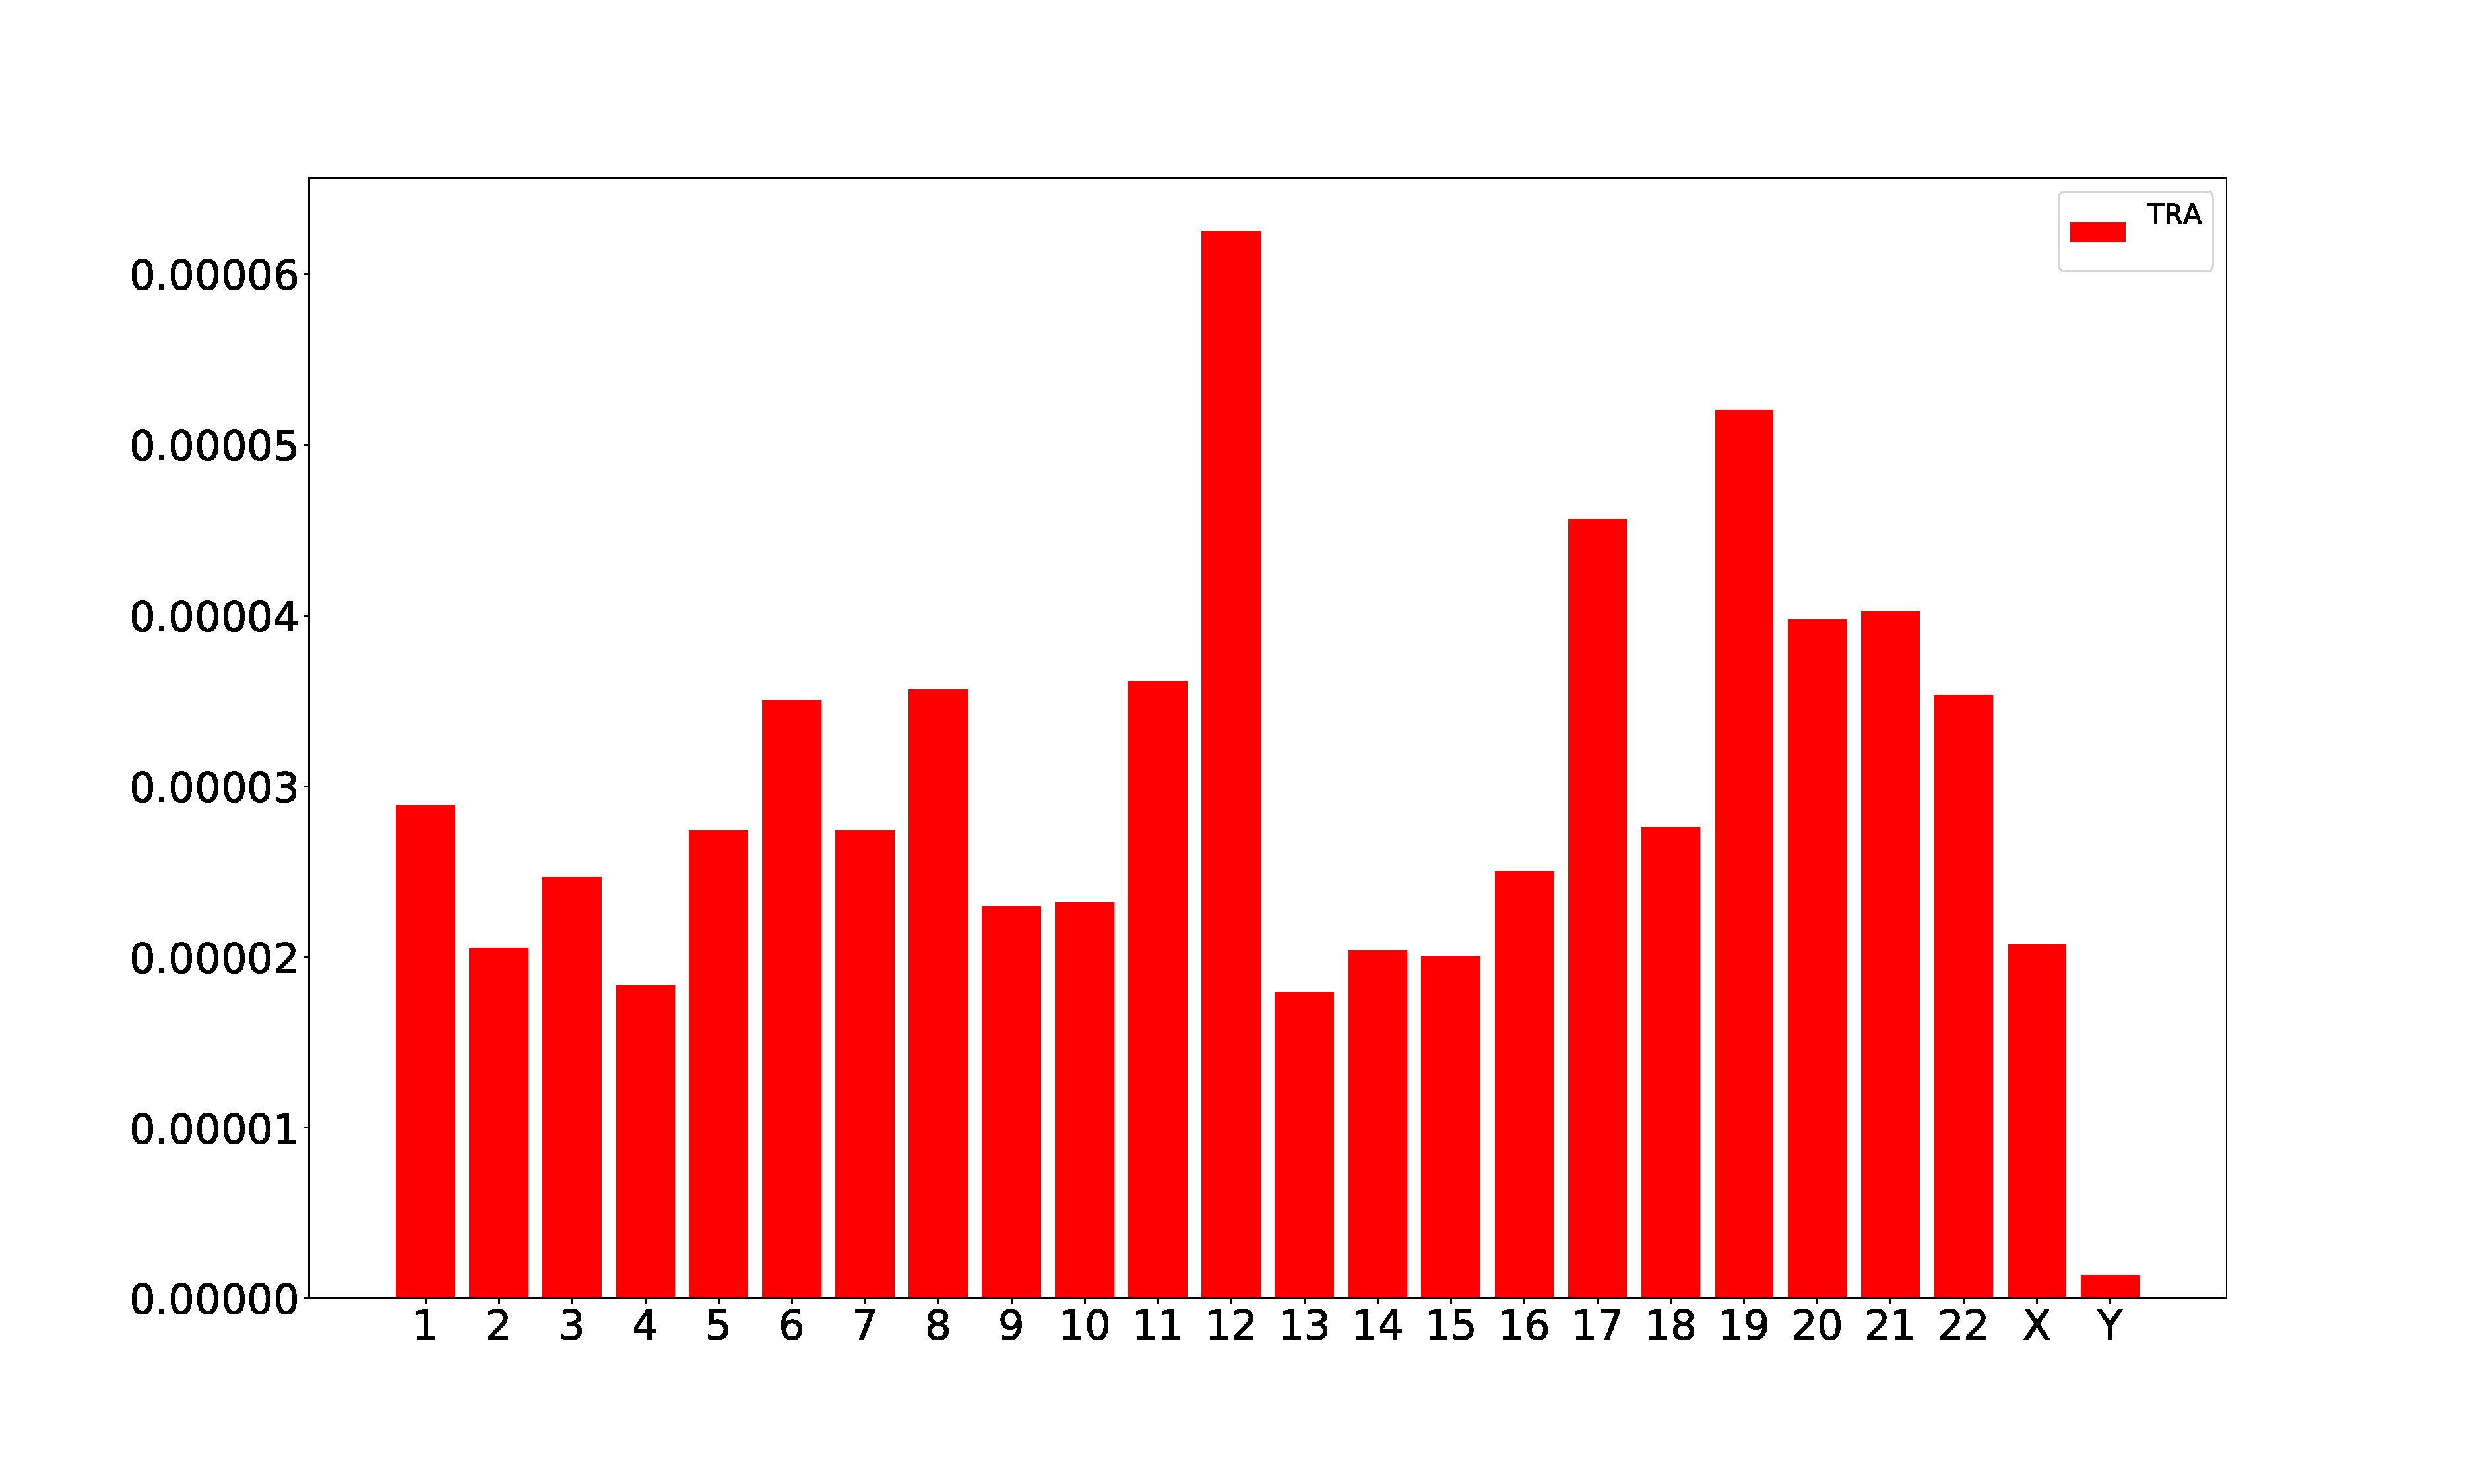
\includegraphics[scale=0.2]{figures/TRA_Break_distribution_normalized.pdf}
\caption{Distribution of TRA breaks per chromosome. Values normalized by chromosome length}
\end{figure}


\pagebreak
\section*{Heat map of break interaction}

To find the most common break pairs, we plot a matrix of frequencies, like a heatmap.


\begin{figure}[H]
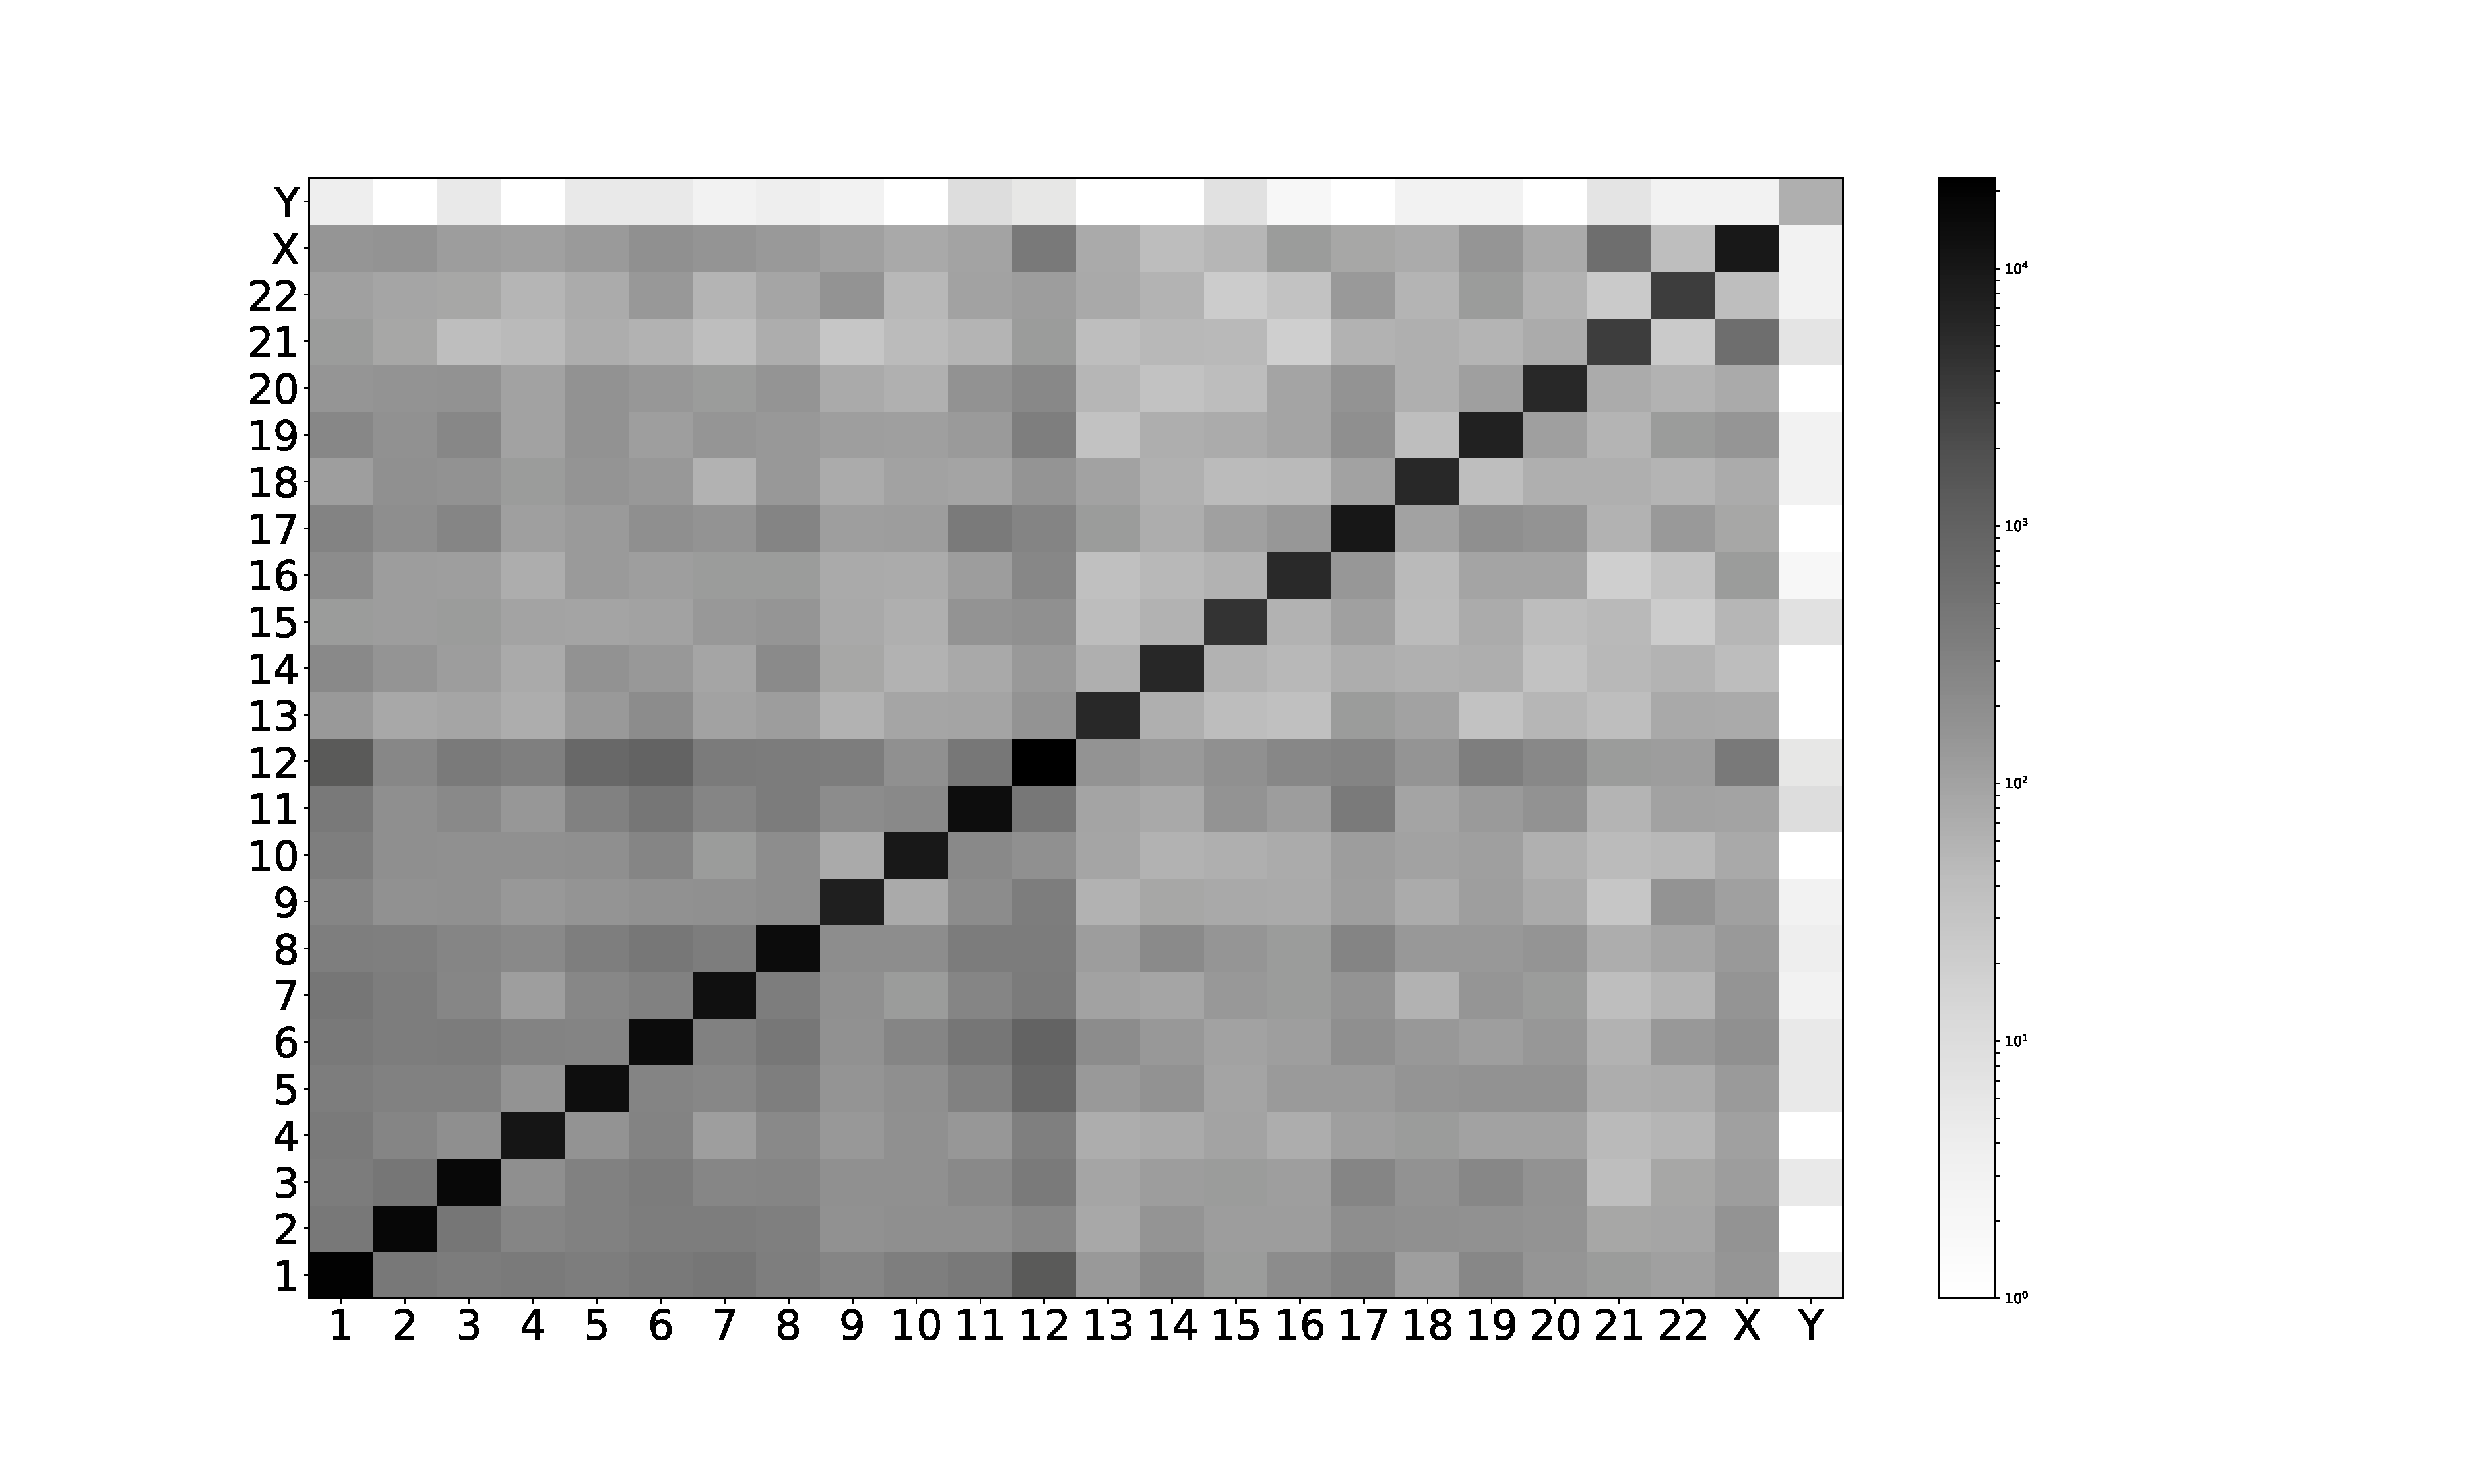
\includegraphics[scale=0.24]{figures/Matrix_break_frequencies_unnormalized.pdf}
\caption{Matrix of break frequencies among chromosomes. Values unnormalized. Logarithmic scale.}
\end{figure}

To clarify, we remove the diagonal, which is dominating the coloring.

\begin{figure}[H]
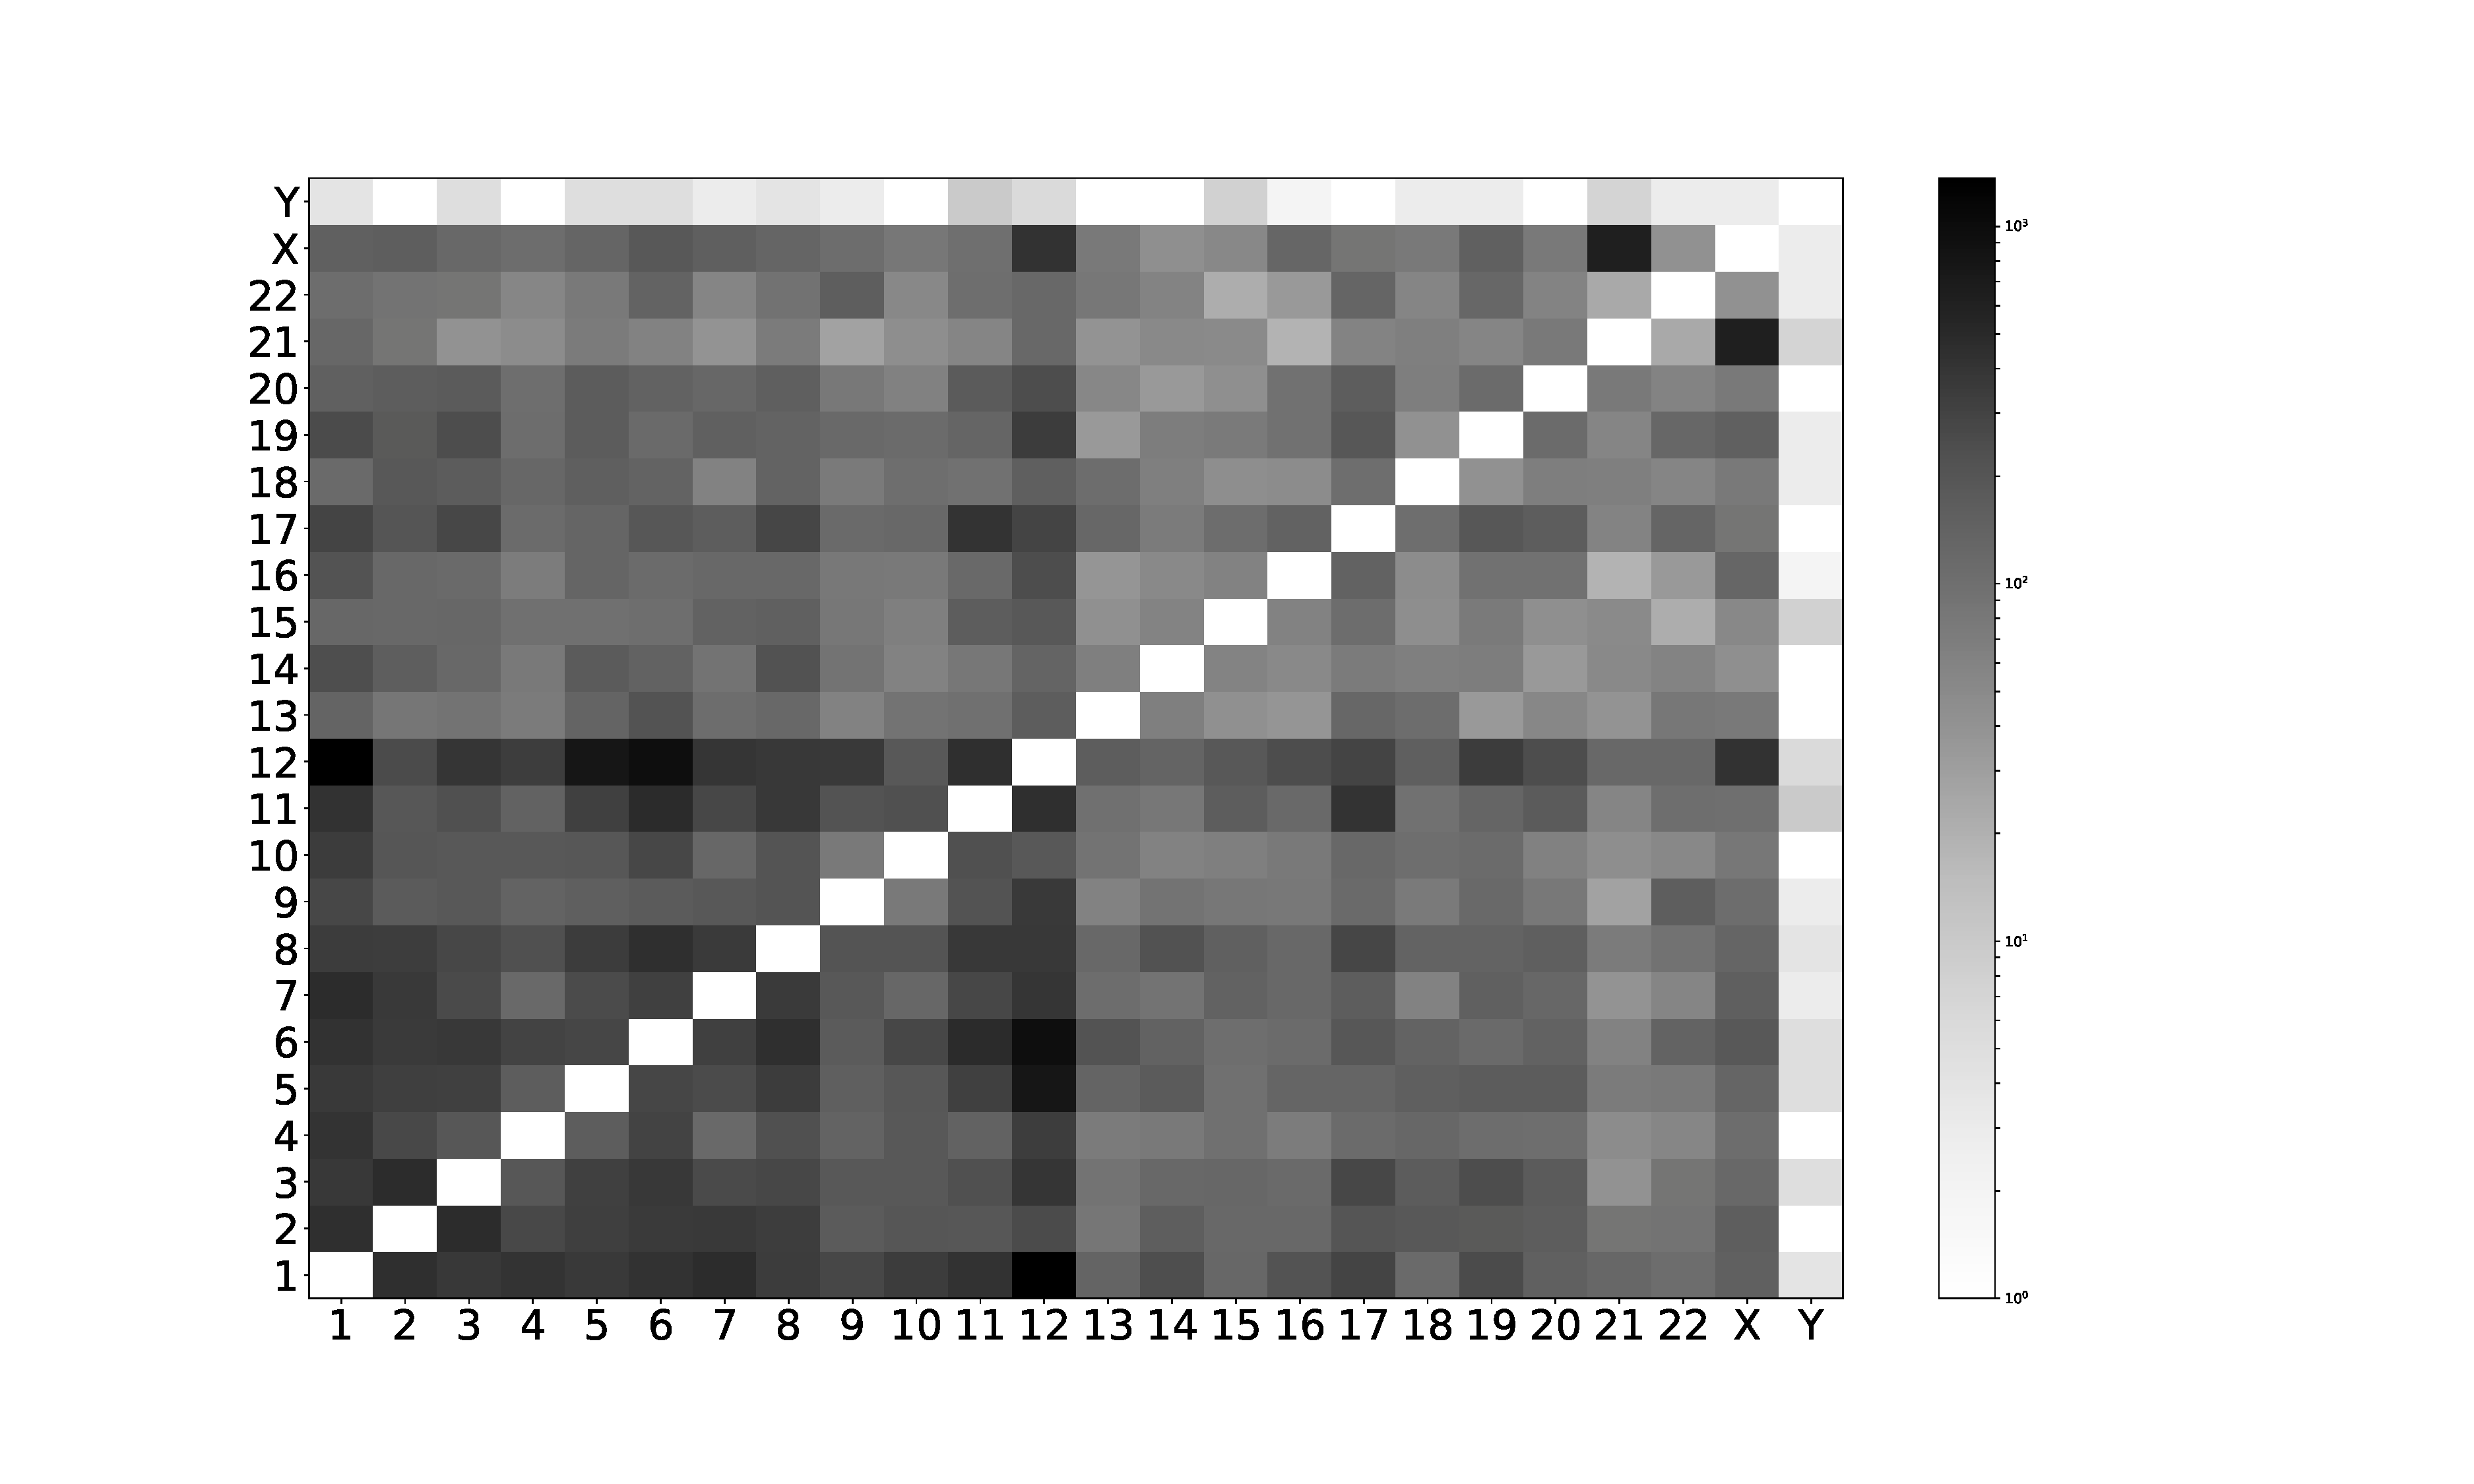
\includegraphics[scale=0.24]{figures/Matrix_break_frequencies_unnormalized_nodiagonal.pdf}
\caption{Matrix of break frequencies among chromosomes. Values unnormalized. Logarithmic scale. Diagonal removed.}
\end{figure}

\subsection*{Heat map of break interaction, normalized}

We normalize the frequencies by the length of both chromosomes involved

\begin{figure}[H]
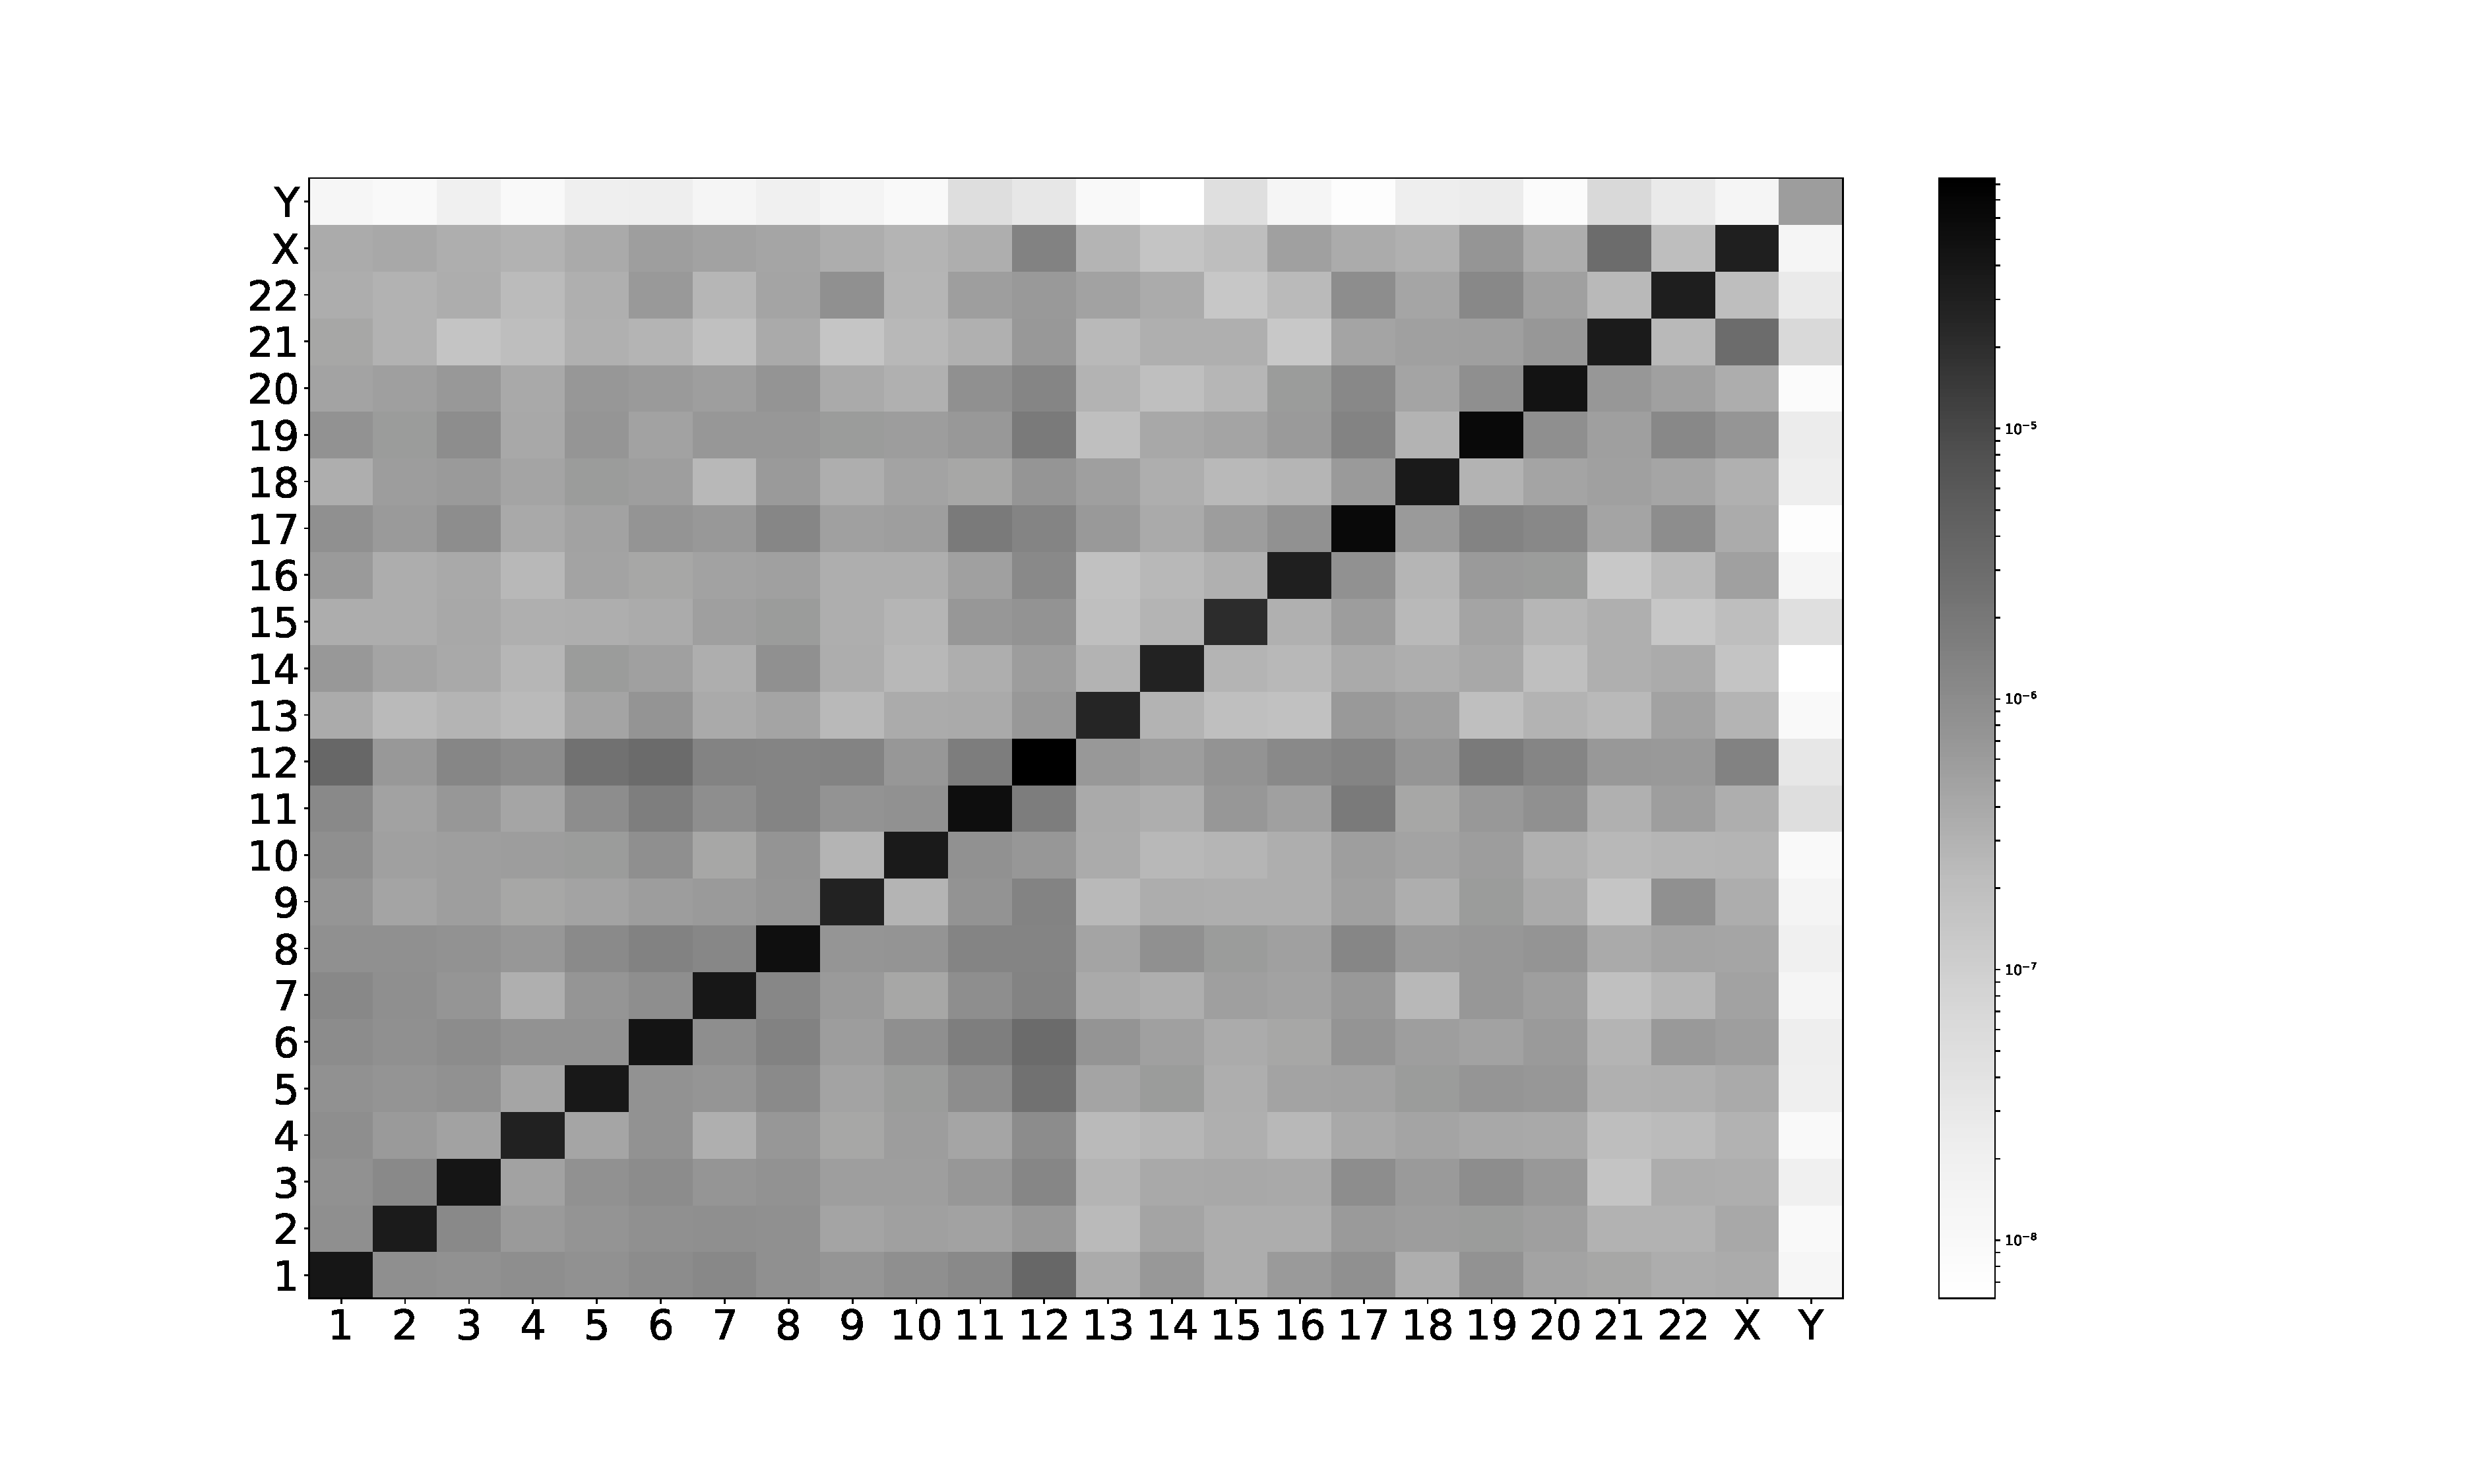
\includegraphics[scale=0.24]{figures/Matrix_break_frequencies_normalized.pdf}
\caption{Matrix of break frequencies among chromosomes. Values normalized by length of the two chromsomes. Logarithmic scale.}
\end{figure}

To clarify, we remove the diagonal, which is dominating the coloring.

\begin{figure}[H]
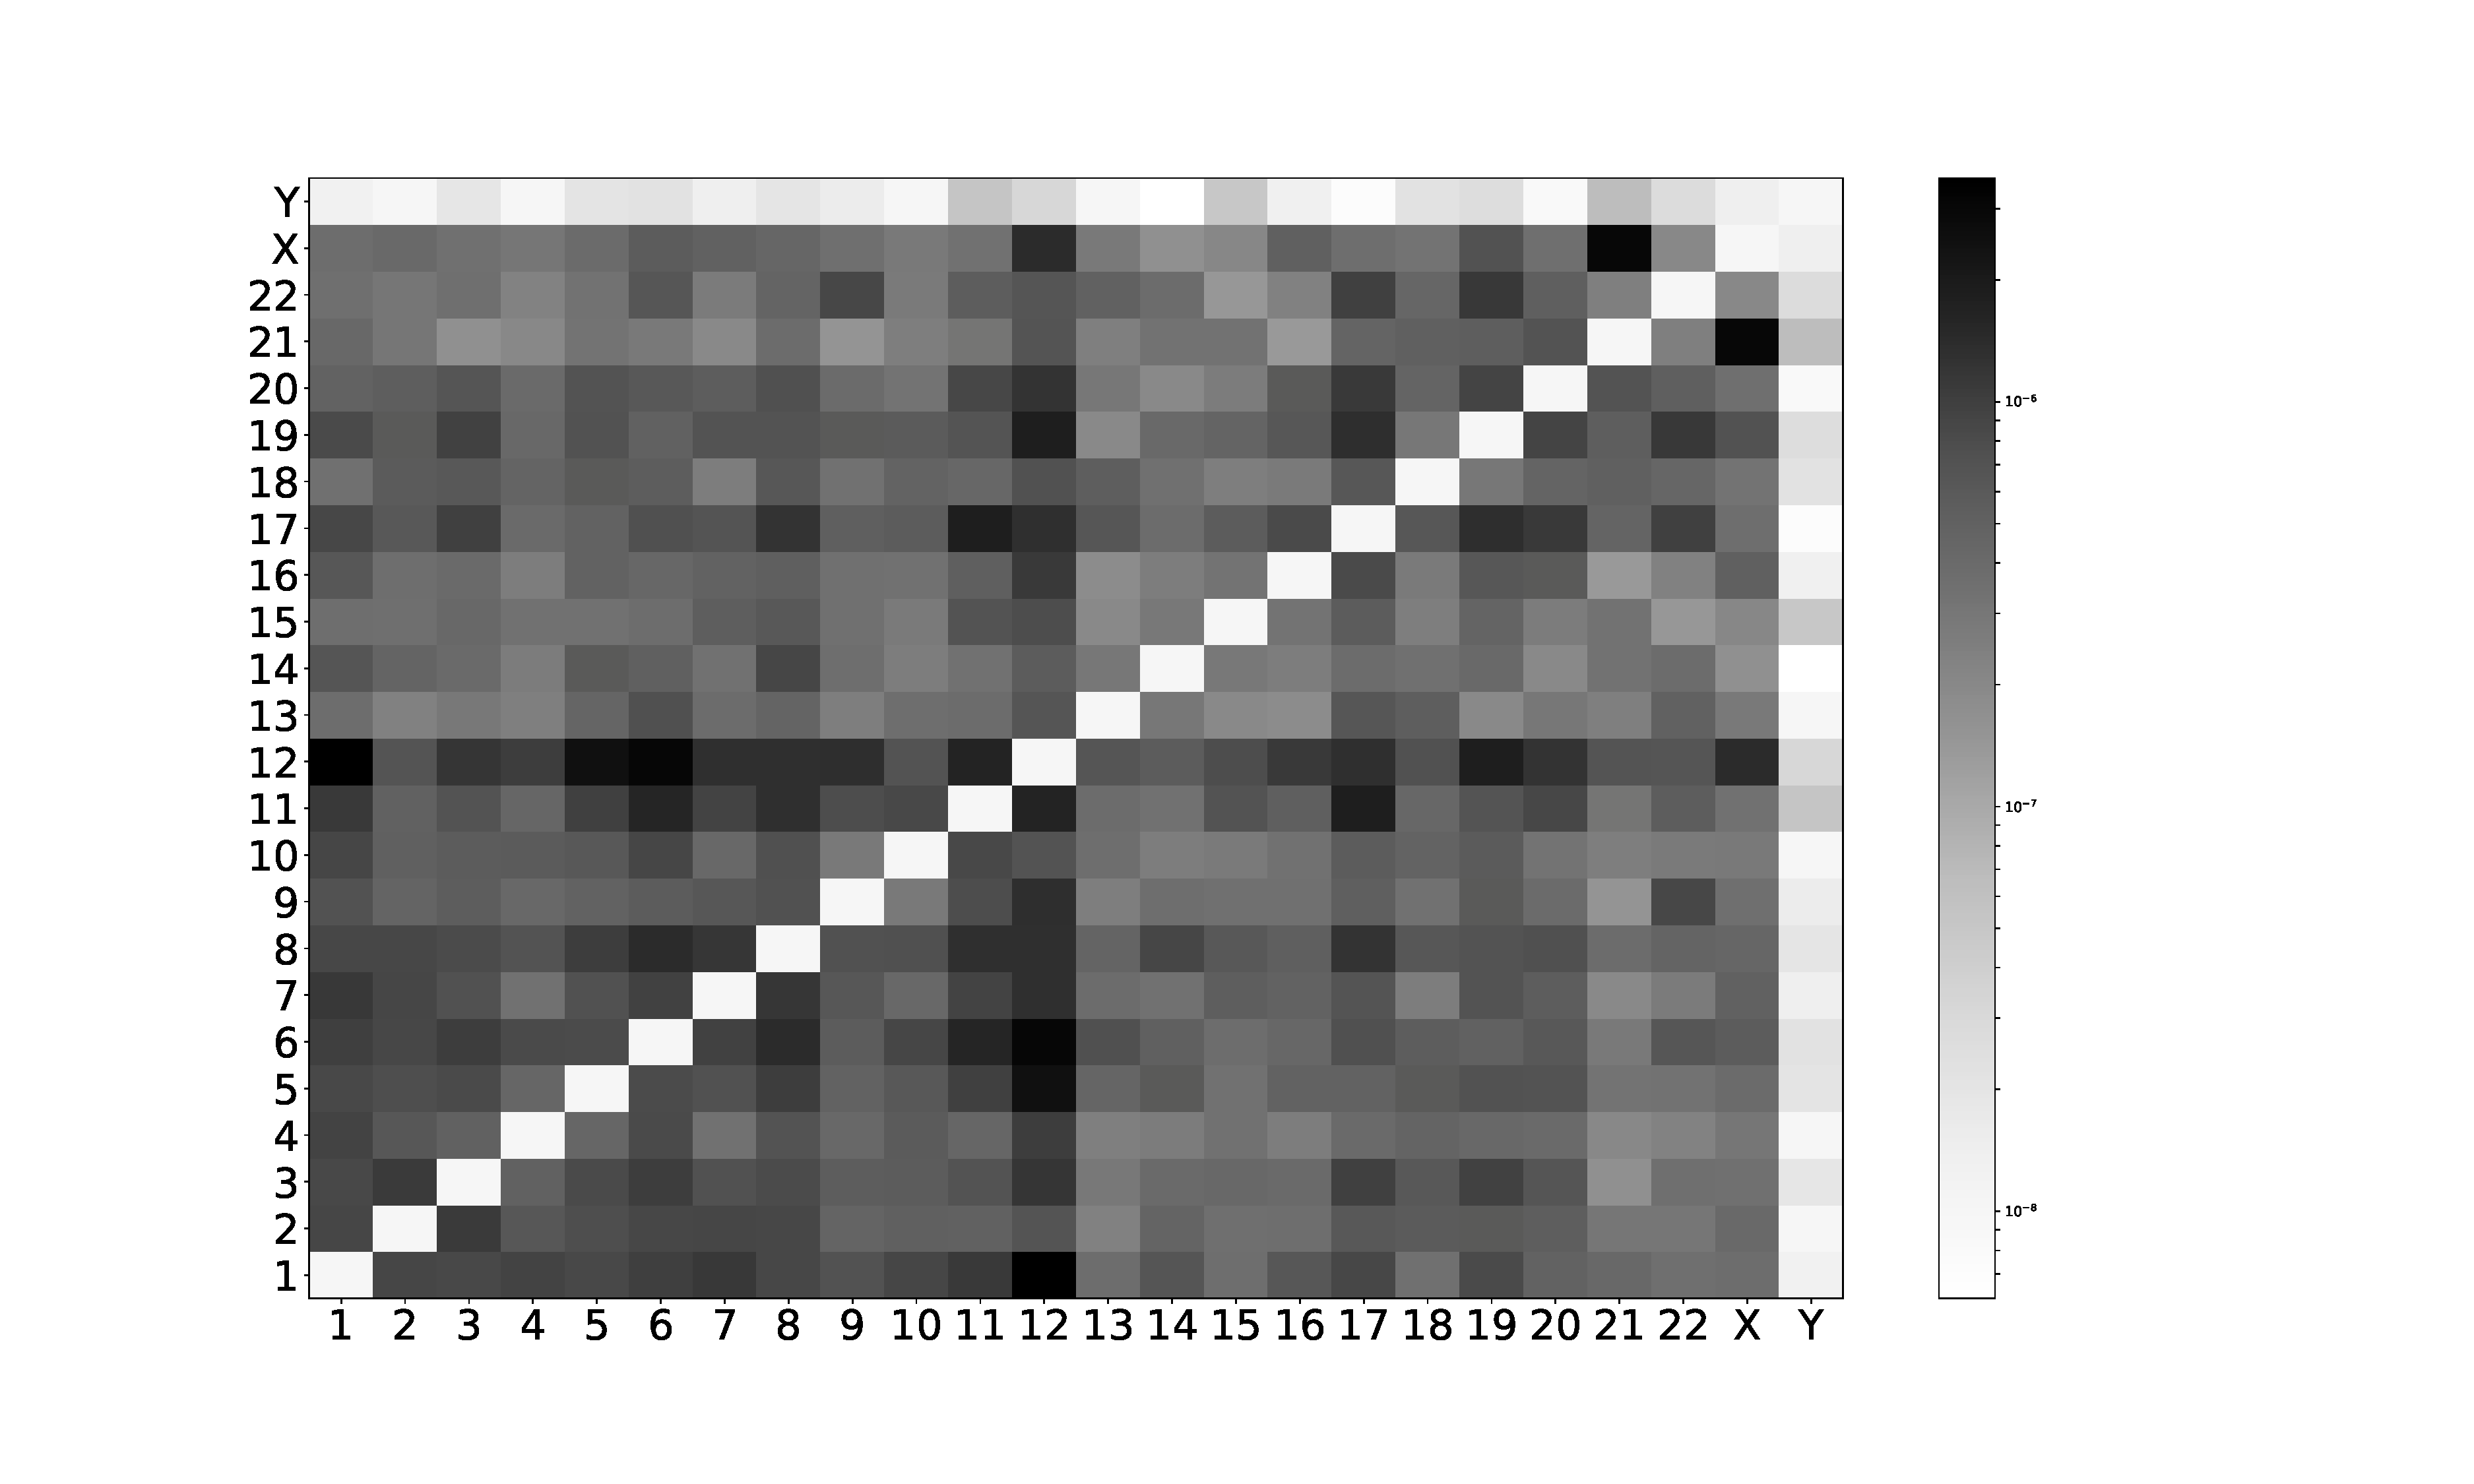
\includegraphics[scale=0.24]{figures/Matrix_break_frequencies_normalized_nodiagonal.pdf}
\caption{Matrix of break frequencies among chromosomes. Values normalized by length of the two chromsomes. Logarithmic scale. Diagonal removed.}
\end{figure}

For reference, we list the top frequencies, avoiding the diagonal:
\begin{enumerate}

\item 12  1
 \item 12  6
 \item 21 23
 \item 12  5
 \item 11 17
 \item 19 12
 \item 12 11
 \item 11  6
 \item 23 12
 \item  8  6
 \item 17 19
 \item 12  9
 \item  7 12
 \item  8 12
 \item 17 12
 \item  8 11
 \item 20 12
 \item 17  8
 \item  3 12
 \item  8  7
 \item  1  7
 \item 22 19
 \item 17 20
 \item 16 12
 \item 11  1
 \item  2  3
 \item  8  5
 \item 12  4
 \item  6  3



\end{enumerate}
\end{document}
